% uWaterloo Thesis Template for LaTeX 
% Last Updated May 24, 2011 by Stephen Carr, IST Client Services
% FOR ASSISTANCE, please send mail to rt-IST-CSmathsci@ist.uwaterloo.ca

% Effective October 2006, the University of Waterloo 
% requires electronic thesis submission. See the uWaterloo thesis regulations at
% http://www.grad.uwaterloo.ca/Thesis_Regs/thesistofc.asp.

% DISCLAIMER
% To the best of our knowledge, this template satisfies the current uWaterloo requirements.
% However, it is your responsibility to assure that you have met all 
% requirements of the University and your particular department.
% Many thanks to the feedback from many graduates that assisted the development of this template.

% -----------------------------------------------------------------------

% By default, output is produced that is geared toward generating a PDF 
% version optimized for viewing on an electronic display, including 
% hyperlinks within the PDF.
 
% To create a PDF output that is optimized for double-sided printing: 
%
% 1) comment-out the \documentclass statement in the preamble below, and
% un-comment the second \documentclass line.
%
% 2) change the value assigned below to the boolean variable
% "PrintVersion" from "false" to "true".

% --------------------- Start of Document Preamble -----------------------

% Specify the document class, default style attributes, and page dimensions
% For hyperlinked PDF, suitable for viewing on a computer, use this:
\documentclass[12pt,titlepage,oneside,final]{book}
 
% For PDF, suitable for double-sided printing, change the PrintVersion variable below
% to "true" and use this \documentclass line instead of the one above:
%\documentclass[12pt,titlepage,openright,twoside,final]{book}

% Some LaTeX commands I define for my own nomenclature.
% If you have to, it's better to change nomenclature once here than in a 
% million places throughout your thesis!
\newcommand{\package}[1]{\textbf{#1}} % package names in bold text
\newcommand{\cmmd}[1]{\textbackslash\texttt{#1}} % command name in tt font 
\newcommand{\href}[1]{#1} % does nothing, but defines the command so the
    % print-optimized version will ignore \href tags (redefined by hyperref pkg).
%\newcommand{\texorpdfstring}[2]{#1} % does nothing, but defines the command
% Anything defined here may be redefined by packages added below...

% This package allows if-then-else control structures.
\usepackage{ifthen}
\newboolean{PrintVersion}
\setboolean{PrintVersion}{false} 
% CHANGE THIS VALUE TO "true" as necessary, to improve printed results for hard copies
% by overriding some options of the hyperref package below.

%\usepackage{nomencl} % For a nomenclature (optional; available from ctan.org)

\usepackage{amsmath,amssymb,amstext} % Lots of math symbols and environments
\usepackage[pdftex]{graphicx} % For including graphics N.B. pdftex graphics driver 
\usepackage{natbib}
\usepackage{graphicx}
\usepackage{subcaption}
\usepackage[space]{grffile}
\usepackage{latexsym}
\usepackage{textcomp}
\usepackage{longtable}
\usepackage{multirow,booktabs}
\usepackage{amsfonts,amsmath,amssymb}
\DeclareMathOperator{\Tr}{trace}
\usepackage{url}
\usepackage{flafter}
\usepackage[all]{nowidow}
\usepackage{parskip}
\usepackage{setspace}
\usepackage{listings}
% \usepackage{breqn}
\lstset{language=Python, breaklines=true} 
\usepackage[utf8]{inputenc}
\usepackage[english]{babel}
\usepackage{caption}
\captionsetup{format=hang}
\usepackage{showlabels}
\usepackage{tabulary}
\usepackage{tabularx}
\usepackage{glossaries}
\makeglossaries
\input{bibliography/glossary.tex}
\usepackage{rotating}
\newcolumntype{Y}{>{\centering\arraybackslash}X}


% Hyperlinks make it very easy to navigate an electronic document.
% In addition, this is where you should specify the thesis title
% and author as they appear in the properties of the PDF document.
% Use the "hyperref" package 
% N.B. HYPERREF MUST BE THE LAST PACKAGE LOADED; ADD ADDITIONAL PKGS ABOVE
\usepackage[pdftex,pagebackref=false]{hyperref} % with basic options
		% N.B. pagebackref=true provides links back from the References to the body text. This can cause trouble for printing.
\hypersetup{
    plainpages=false,       % needed if Roman numbers in frontpages
    % pdfpagelabels=true,     % adds page number as label in Acrobat's page count
    % bookmarks=true,         % show bookmarks bar?
    unicode=false,          % non-Latin characters in Acrobat’s bookmarks
    pdftoolbar=true,        % show Acrobat’s toolbar?
    pdfmenubar=true,        % show Acrobat’s menu?
    pdffitwindow=false,     % window fit to page when opened
    pdfstartview={FitH},    % fits the width of the page to the window
    pdftitle={uWaterloo\ LaTeX\ Thesis\ Template},    % title: CHANGE THIS TEXT!
    pdfauthor={Mike Yetisir},    % author: CHANGE THIS TEXT! and uncomment this line
    pdfsubject={Up-Scaling Discrete Element Method Simulations of Discontinua},  % subject: CHANGE THIS TEXT! and uncomment this line
%    pdfkeywords={Up-Scaling} {Multi-scale} {Homogenization} {DEM}, % list of keywords, and uncomment this line if desired
    pdfnewwindow=true,      % links in new window
    colorlinks=true,        % false: boxed links; true: colored links
    linkcolor=blue,         % color of internal links
    citecolor=green,        % color of links to bibliography
    filecolor=magenta,      % color of file links
    urlcolor=cyan           % color of external links
}
\ifthenelse{\boolean{PrintVersion}}{   % for improved print quality, change some hyperref options
\hypersetup{	% override some previously defined hyperref options
%    colorlinks,%
    citecolor=black,%
    filecolor=black,%
    linkcolor=black,%
    urlcolor=black}
}{} % end of ifthenelse (no else)

% Setting up the page margins...
% uWaterloo thesis requirements specify a minimum of 1 inch (72pt) margin at the
% top, bottom, and outside page edges and a 1.125 in. (81pt) gutter
% margin (on binding side). While this is not an issue for electronic
% viewing, a PDF may be printed, and so we have the same page layout for
% both printed and electronic versions, we leave the gutter margin in.
% Set margins to minimum permitted by uWaterloo thesis regulations:
\setlength{\marginparwidth}{0pt} % width of margin notes
% N.B. If margin notes are used, you must adjust \textwidth, \marginparwidth
% and \marginparsep so that the space left between the margin notes and page
% edge is less than 15 mm (0.6 in.)
\setlength{\marginparsep}{0pt} % width of space between body text and margin notes
\setlength{\evensidemargin}{0.125in} % Adds 1/8 in. to binding side of all 
% even-numbered pages when the "twoside" printing option is selected
\setlength{\oddsidemargin}{0.125in} % Adds 1/8 in. to the left of all pages
% when "oneside" printing is selected, and to the left of all odd-numbered
% pages when "twoside" printing is selected
\setlength{\textwidth}{6.375in} % assuming US letter paper (8.5 in. x 11 in.) and 
% side margins as above
\raggedbottom

% The following statement specifies the amount of space between
% paragraphs. Other reasonable specifications are \bigskipamount and \smallskipamount.
\setlength{\parskip}{\medskipamount}

% The following statement controls the line spacing.  The default
% spacing corresponds to good typographic conventions and only slight
% changes (e.g., perhaps "1.2"), if any, should be made.
\renewcommand{\baselinestretch}{1.1} % this is the default line space setting

% By default, each chapter will start on a recto (right-hand side)
% page.  We also force each section of the front pages to start on 
% a recto page by inserting \cleardoublepage commands.
% In many cases, this will require that the verso page be
% blank and, while it should be counted, a page number should not be
% printed.  The following statements ensure a page number is not
% printed on an otherwise blank verso page.
\let\origdoublepage\cleardoublepage
\newcommand{\clearemptydoublepage}{%
  \clearpage{\pagestyle{empty}\origdoublepage}}
\let\cleardoublepage\clearemptydoublepage

%======================================================================
%   L O G I C A L    D O C U M E N T -- the content of your thesis
%======================================================================
\begin{document}

%----------------------------------------------------------------------
% FRONT MATTER
%----------------------------------------------------------------------
% T I T L E   P A G E
% -------------------
% Last updated May 24, 2011, by Stephen Carr, IST-Client Services
% The title page is counted as page `i' but we need to suppress the
% page number.  We also don't want any headers or footers.
\pagestyle{empty}
\pagenumbering{roman}

% The contents of the title page are specified in the "titlepage"
% environment.
\begin{titlepage}
        \begin{center}
        \vspace*{1.0cm}

        \Huge
        {\bf Up-Scaling Discrete Element Method Simulations of Discontinua}

        \vspace*{1.0cm}

        \normalsize
        by \\

        \vspace*{1.0cm}

        \Large
        Mike Yetisir \\

        \vspace*{3.0cm}

        \normalsize
        A thesis \\
        presented to the University of Waterloo \\ 
        in fulfillment of the \\
        thesis requirement for the degree of \\
        Master of Applied Science \\
        in \\
        Civil Engineering \\

        \vspace*{2.0cm}

        Waterloo, Ontario, Canada, 2016 \\

        \vspace*{1.0cm}

        \copyright\ Mike Yetisir 2016 \\
        \end{center}
\end{titlepage}

% The rest of the front pages should contain no headers and be numbered using Roman numerals starting with `ii'
\pagestyle{plain}
\setcounter{page}{2}

\cleardoublepage % Ends the current page and causes all figures and tables that have so far appeared in the input to be printed.
% In a two-sided printing style, it also makes the next page a right-hand (odd-numbered) page, producing a blank page if necessary.
 


% D E C L A R A T I O N   P A G E
% -------------------------------
  % The following is the sample Delaration Page as provided by the GSO
  % December 13th, 2006.  It is designed for an electronic thesis.
  \noindent
I hereby declare that I am the sole author of this thesis. This is a true copy of the thesis, including any required final revisions, as accepted by my examiners.

  \bigskip
  
  \noindent
I understand that my thesis may be made electronically available to the public.

\cleardoublepage
%\newpage

% A B S T R A C T
% ---------------

\begin{center}\textbf{Abstract}\end{center}

Pre-existing fractures significantly influence the geomechanical response of the rock mass at the reservoir scale. For geomechanical applications, these natural fractures need to be considered in the mechanical response of the system. Distinct Element Methods (DEM) are often used to explicitly model the mechanics of Naturally Fractured Rock (NFR); however, they are often too computationally prohibitive for reservoir-scale problems. A DEM up-scaling framework is presented that facilitates estimating a representative parameter set for continuum constitutive models that capture the salient feature of Naturally Fractured Rock (NFR) behaviour. 

Up-scaling is achieved by matching homogenized DEM stress-strain curves from multiple load paths to those of continuum constitutive models using a Particle Swarm Optimization (PSO) algorithm followed by a Damped Least-Squares (DLS) algorithm. The effectiveness of the framework is demonstrated by up-scaling a DEM model of a NFR to a Drucker-Prager damage-plasticity model; the up-scaled model is shown to capture well the effect of confinement on the the yielding and sliding of natural fractures in the rock mass. 

The goal of this thesis is to present a framework to facilitate effective simulation of fine-scale behaviour in full-scale NFR systems while significantly reducing the computational demands associated with modelling these systems with DEM. 

As such, four main research objectives have been identified and achieved: 1) Develop and implement stress and strain homogenization algorithms for DEM models with deformable blocks, 2) present a methodology to parameterize complex nonlinear continuum constitutive models, 3) develop and implement an automated modular software framework for up-scaling DEM simulations, and 4) demonstrate that the performance of the up-scaled continuum models are accurate and significantly more computationally efficient.

The up-scaling methodology is verified through a case study on a naturally fractured granite slope in which the top surface is loaded until failure. The up-scaled continuum model is shown to compare quite well to Direct Numerical Simulation (DNS) in a slope stability analysis and requires two orders of magnitude less computational effort.

\cleardoublepage
%\newpage

% A C K N O W L E D G E M E N T S
% -------------------------------

\begin{center}\textbf{Acknowledgements}\end{center}

This thesis, though perhaps at times a lonely affair, could not have been possible without the involvement and support of many individuals who helped and encouraged me at every step along the way. I wish to acknowledge the invaluable support and contributions that everyone provided. 

First and foremost, I wish to thank my two research supervisors, Dr. Rob Gracie and Dr. Maurice Dusseault, for their endless technical insights, inspirational ideas, and moral support throughout the duration of this degree. Without their guidance, this research thesis would not have been nearly as comprehensive nor comprehensible.

Additionally, I would like to acknowledge Dr. L. Shawn Matott for allowing me to use his OSTRICH optimization software and providing some much needed support when I was getting started. 

Furthermore, I should thank my partners in crime (and research), Endrina Rivas and Eleanor Mak, with whom I have shared many late nights at the office. These ladies have kept me motivated when my research has stagnated, while conversely making sure I never worked too hard. 

Lastly, additional thanks goes to my coaches, Vinit Kudva, Clive Porter, and Jeff Muirhead for pushing me to be my best on and off the court, distracting me from my studies, and allowing me to be part of such a wonderfull team.

\cleardoublepage
%\newpage

% % D E D I C A T I O N
% % -------------------

% \begin{center}\textbf{Dedication}\end{center}

% This thesis is dedicated to

% \cleardoublepage
% %\newpage

% T A B L E   O F   C O N T E N T S
% ---------------------------------
\renewcommand\contentsname{Table of Contents}
\tableofcontents
\cleardoublepage
\phantomsection
%\newpage

% L I S T   O F   T A B L E S
% ---------------------------
\addcontentsline{toc}{chapter}{List of Tables}
\listoftables
\cleardoublepage
\phantomsection		% allows hyperref to link to the correct page
%\newpage

% L I S T   O F   F I G U R E S
% -----------------------------
\addcontentsline{toc}{chapter}{List of Figures}
\listoffigures
\cleardoublepage
\phantomsection		% allows hyperref to link to the correct page
%\newpage

% L I S T   O F   S Y M B O L S
% -----------------------------
%To include a Nomenclature section
\addcontentsline{toc}{chapter}{List of Abbreviations}
\setlength{\glslistdottedwidth}{0.4\textwidth}
\printglossary[title={List of Abbreviations}, style=listdotted, nogroupskip]
\cleardoublepage
\phantomsection % allows hyperref to link to the correct page
%\newpage

% Change page numbering back to Arabic numerals
\pagenumbering{arabic}

 

%----------------------------------------------------------------------
% CHAPTER 1
%----------------------------------------------------------------------
\input{Chapter1} 

%----------------------------------------------------------------------
% CHAPTER 2
%----------------------------------------------------------------------
%\input{Chapter2} 

%----------------------------------------------------------------------
% CHAPTER 3
%----------------------------------------------------------------------
%======================================================================
\chapter{Up-Scaling Methodology}
%======================================================================

The goal of the following up-scaling methodology is to identify the parameters of a continuum constitutive model (macroscale model) that best emulates the average response in the \acrshort{dem} \acrfull{rev} (microscale model). Let the displacement, strain and stress of the \acrshort{dem} \acrshort{rev} (microscale) model be denoted by $\mathbf{u}^m$, $\boldsymbol{\epsilon}^m$, and $\boldsymbol{\sigma}^m$, respectively. Let the homogenized (averaged) strain and stress in the \acrshort{dem} \acrshort{rev} model be denoted by  $\left<\boldsymbol{\epsilon}\right>$ and $\left<\boldsymbol{\sigma}\right>$, respectively.  Finally, let the strain and stress from the continuum (macroscale) constitutive model be denoted as $\boldsymbol{\epsilon}^M$ and $\boldsymbol{\sigma}^M$, respectively. The rate of macroscale stress, $\dot{\boldsymbol{\sigma}}^M=\dot{\boldsymbol{\sigma}}^M\left(\dot{\boldsymbol{\epsilon}}^M, \boldsymbol{\chi},\mathbf{h}\right)$, is defined in terms of the rate of macroscale strain, $\dot{\boldsymbol{\epsilon}}^M$, a set of material parameters $\boldsymbol{\chi}$ and a set of internal history variables $\mathbf{h}$.

The up-scaling methodology has five steps: 
\begin{enumerate}
    \item Identify the \acrshort{dem} \acrshort{rev} for the \acrshort{nfr}.
	\item Exercise the \acrshort{dem} \acrshort{rev} using multiple load paths. Store $\mathbf{u}^m$, $\boldsymbol{\epsilon}^m$, and $\boldsymbol{\sigma}^m$ for each load path.
	\item Apply homogenization algorithms to the microscale results ($\mathbf{u}^m$, $\boldsymbol{\epsilon}^m$, and $\boldsymbol{\sigma}^m$) to determine the average stress-strain response of the \acrshort{rev}, i.e., $\left<\boldsymbol{\sigma}\right>$-$\left<\boldsymbol{\epsilon}\right>$, for each load path.
	\item Identify a continuum constitutive model, $\dot{\boldsymbol{\sigma}}^M=\dot{\boldsymbol{\sigma}}^M\left(\dot{\boldsymbol{\epsilon}}^M, \boldsymbol{\chi},\mathbf{h}\right)$, that captures the salient features of \acrshort{nfr} mechanics.
	\item Run parameter estimation algorithms to identify the parameters, $\boldsymbol{\chi}$, that minimize the difference between $\left<\boldsymbol{\sigma}\right>$-$\left<\boldsymbol{\epsilon}\right>$ and $\boldsymbol{\sigma}^M$-$\boldsymbol{\epsilon}^M$ over all load paths.
\end{enumerate}

Once an optimal parameter set, $\boldsymbol{\chi}$, for the desired model, $\dot{\boldsymbol{\sigma}}^M=\dot{\boldsymbol{\sigma}}^M\left(\dot{\boldsymbol{\epsilon}}^M, \boldsymbol{\chi},\mathbf{h}\right)$, has been identified, the newly established constitutive model can be used in \acrfull{fem} models or with other suitable numerical or analytical simulations.

%----------------------------------------------------------------------
\section{Up-Scaling Implementation Overview}
%----------------------------------------------------------------------

The up-scaling framework consists of four main software components (Figure \ref{fig:workflow}): a \acrshort{dem} simulator, a homogenization module, a \acrfull{fem} simulator, and a parameter estimation module. In procedural order, the first software component involved is a \acrshort{dem} simulation package, which is used to directly model the \acrshort{nfr}. 

\begin{figure}[p]
\begin{center}
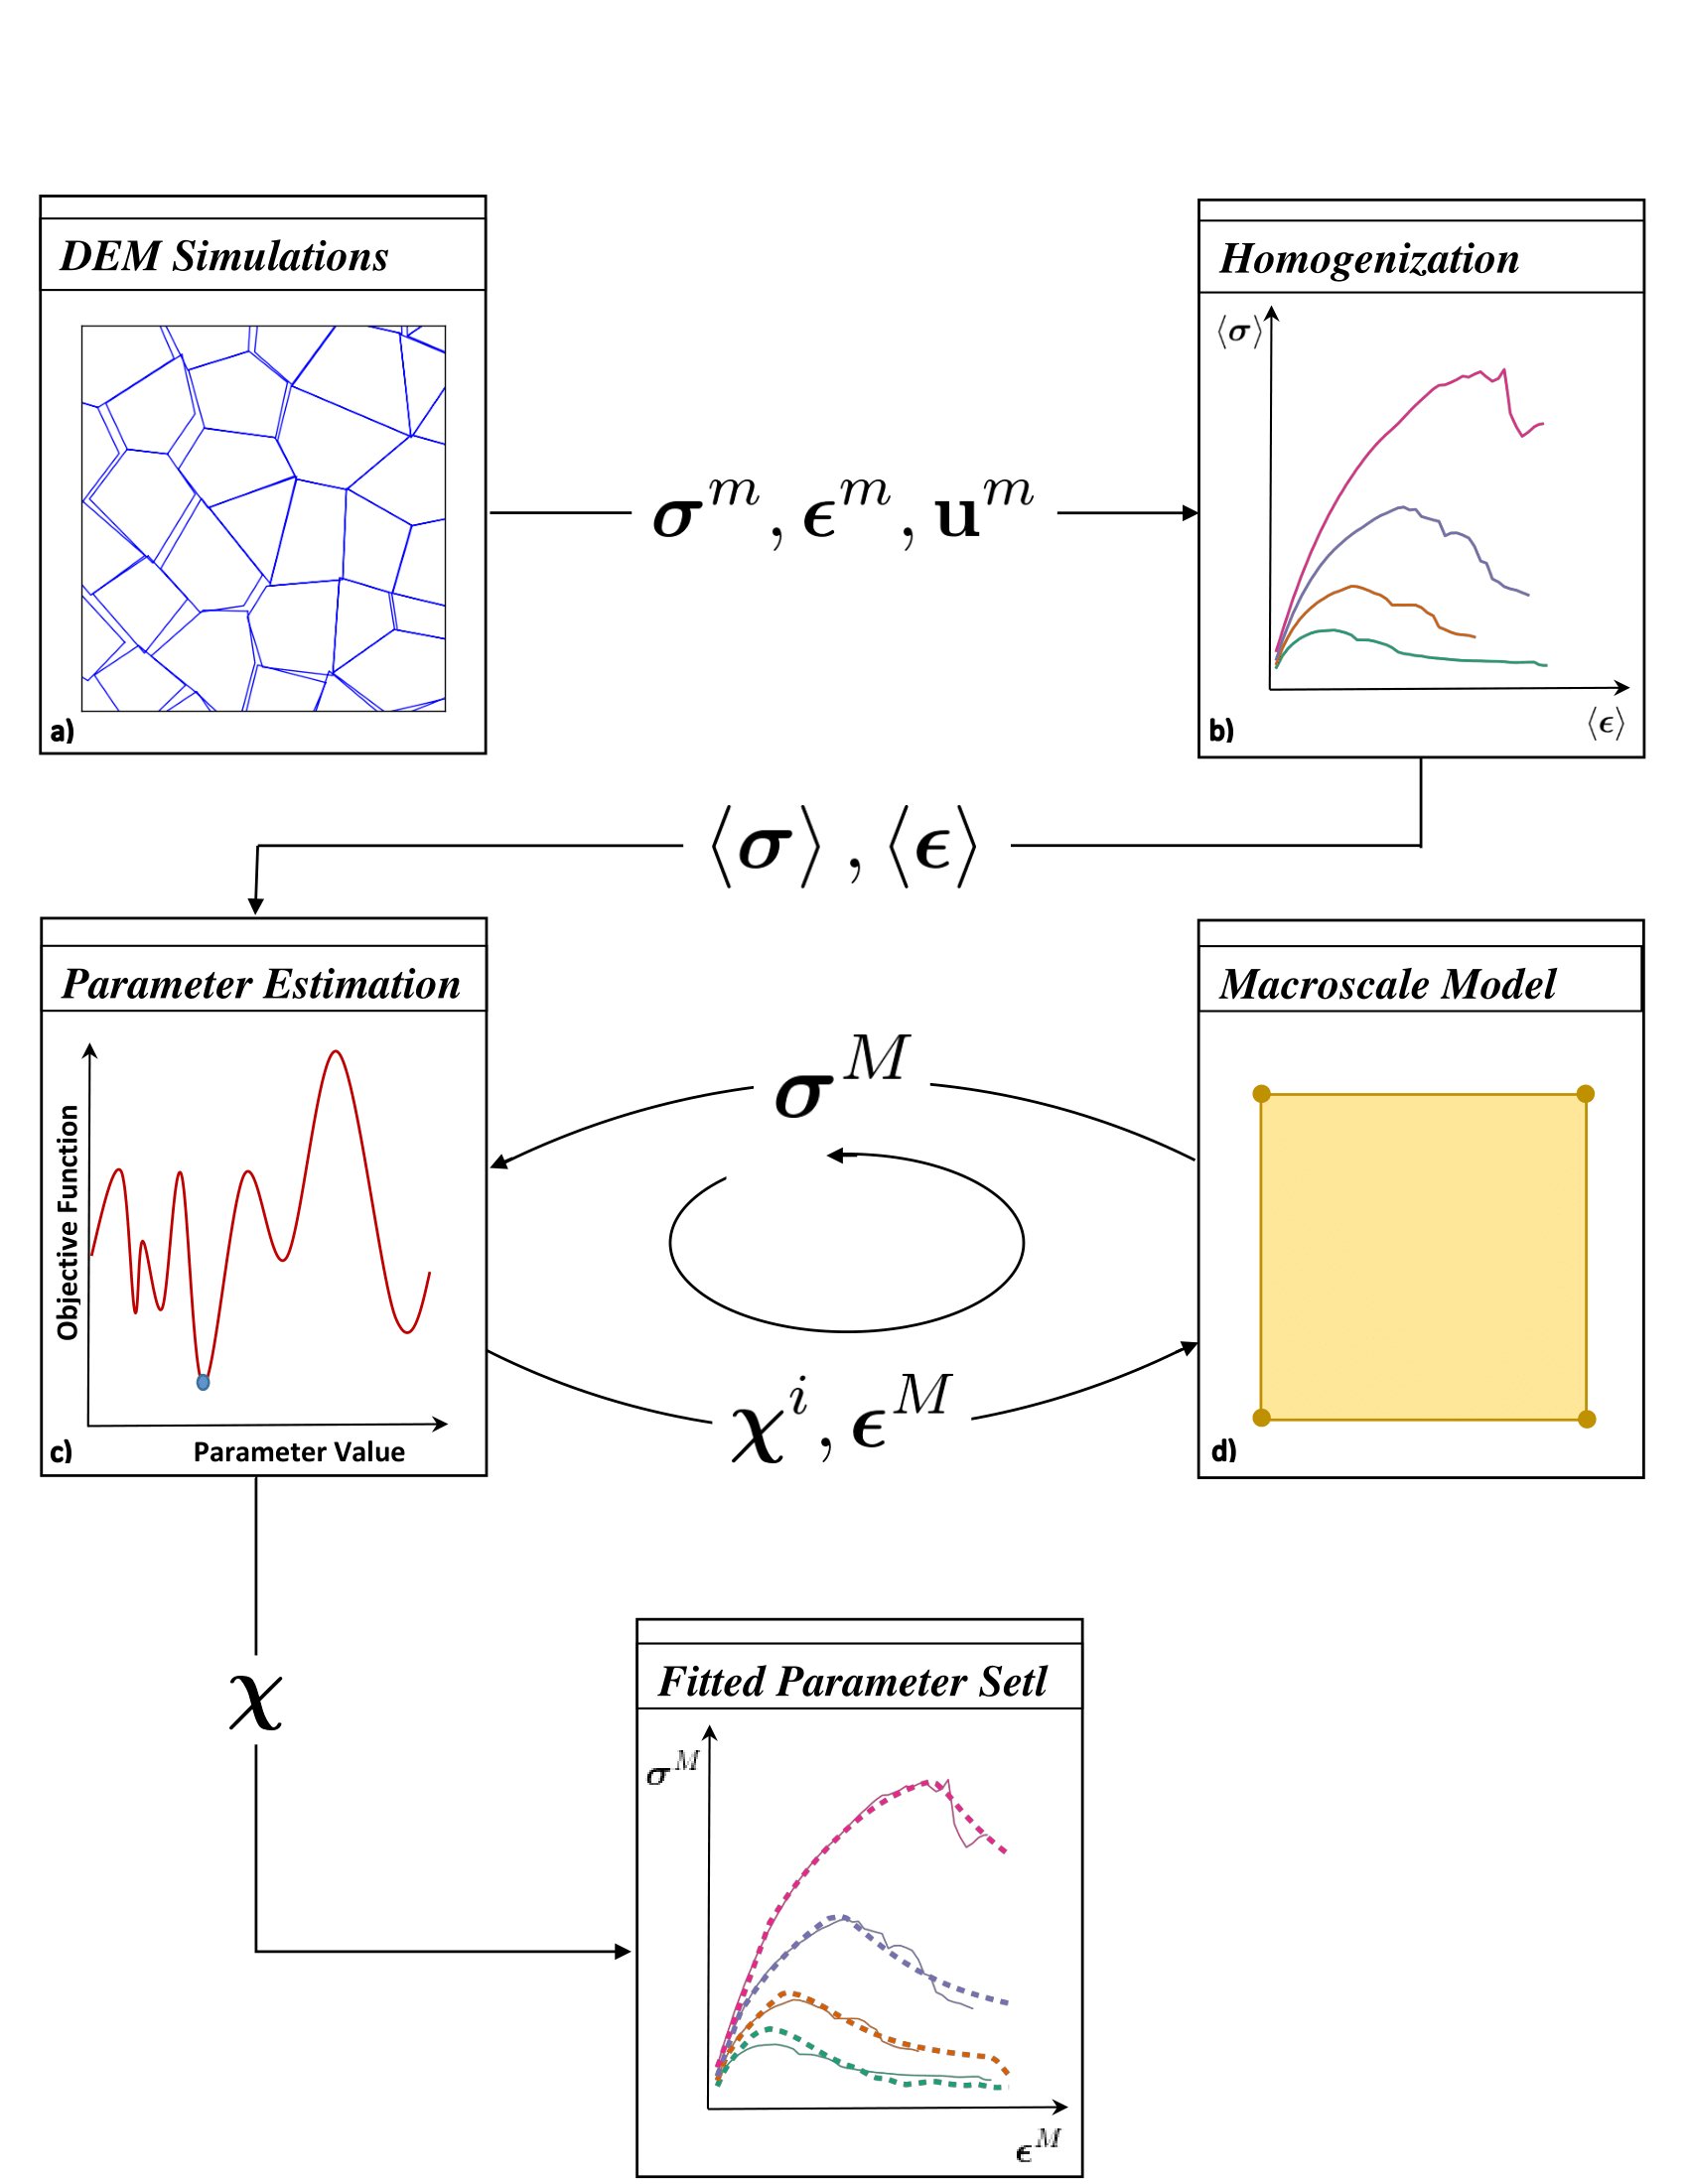
\includegraphics[width=0.75\textwidth]{figures/Chapter3/UpScalingFlowChart}
\caption{{\label{fig:workflow}Up-scaling workflow used to estimate the optimal continuum model parameter set. The DEM software (a) produces a data set which is run through homogenization software (b) which in turn produces another dataset that is fed into the parameter estimation program (c). This parameter estimation program drives the macroscale simulations (d) iteratively in order to find an optimal parameter set for the fitted model.
}}
\end{center}
\end{figure}

The \acrshort{dem} software accepts as inputs the geometry of the \acrshort{dfn}, the material properties of the rock and the natural fractures, and the load paths. The \acrshort{dem} \acrshort{rev} is exercised for different load-paths in a way that is akin to conducting multiple triaxial tests on physical specimens to characterize the full range of material behaviour. The \acrshort{dem} software outputs the microscale displacement, $\mathbf{u}^m$, and stress-strain, $\boldsymbol{\sigma}^m$-$\boldsymbol{\epsilon}^m$, responses for each load path.  This microscale data is subsequently fed into the homogenization module to compute the average stress-strain response, $\left<\boldsymbol{\sigma}\right>$-$\left<\boldsymbol{\epsilon}\right>$,  for each load path. Next, the homogenized stress-strain data, $\left<\boldsymbol{\sigma}\right>$-$\left<\boldsymbol{\epsilon}\right>$, is used by the parameter estimation software as observation data (i.e., laboratory/field data). The parameter estimation module iteratively executes a constitutive model, $\dot{\boldsymbol{\sigma}}^M=\dot{\boldsymbol{\sigma}}^M\left(\dot{\boldsymbol{\epsilon}}^M, \boldsymbol{\chi},\mathbf{h}\right)$, embedded in the \acrshort{fem} simulator for each load path using different parameter sets, $\boldsymbol{\chi}^i$, while attempting to minimize the error between the homogenized microscale, $\left<\boldsymbol{\sigma}\right>$-$\left<\boldsymbol{\epsilon}\right>$, and macroscale, $\boldsymbol{\sigma}^M$-$\boldsymbol{\epsilon}^M$,  stress-strain curves. Eventually, the algorithm converges to a near-optimal parameter set, $\boldsymbol{\chi}$, that can be viewed to be the best estimate of the NFR responses by the given continuum model. 

In my implementation, UDEC\textsuperscript{TM} was used as the \acrshort{dem} simulator and ABAQUS\textsuperscript{TM} was used as the \acrshort{fem} simulator. In ABAQUS\textsuperscript{TM}, single element simulations were performed with a strain-history prescribed through displacement boundary conditions for a given set of material parameters and the stress is obtained as the output. There is nothing particularly special about the \acrshort{dem} or \acrshort{fem} simulators chosen; each could easily be replaced to overcome any inherent limitations.  Moreover, a \acrshort{fem} simulator is not actually needed, since its inclusion in this framework is simply to gain access to the constitutive models within. The \acrshort{fem} simulator could easily be replaced by a \acrfull{fdm} simulator or simply by a material subroutine.  OSTRICH\textsuperscript{TM}, a model-independent optimization package \citep{matott_ostrich:_2016}, is used for the parameter estimation module. I implemented the homogenization module in Python\textsuperscript{TM}. I also used Python\textsuperscript{TM} to develop interfaces drive the various components of the up-scaling framework.

%----------------------------------------------------------------------
\section{Distinct Element Method}
%----------------------------------------------------------------------

Discontinuous systems are characterized by the existence of discontinuities that separate discrete domains within the system. In order to effectively model a discontinuous system, it is necessary to represent two distinct types of mechanical behaviour: the behaviour of the discontinuities and the behaviour of the solid material.

There exists a set of methods, referred to as discrete element methods, which provide the capacity to explicitly represent the behaviour of multiple intersecting discontinuities. The methods allow for the modelling of finite displacements and rotations of discrete bodies, including contact detachment as well as automatic detection of new contacts. Within the set of Discrete Element Methods, there are four subsets \citep{CUNDALL_1992}: Modal Methods, Discontinuous Deformation Analysis Methods, Momentum Exchange Methods, and \acrfull{dem}. In this thesis, the discrete element method used is \acrshort{dem}.

With \acrshort{dem} methods, the discontinuous system is represented as an assembly of deformable blocks such that the interfaces between the blocks represent the discontinuities. With respect to NFR, the blocks can be used to represent the intact rock while the discontinuities represent the joints in the rock mass. 

Consider an arbitrary deformable domain, $\Omega$, with a boundary, $\Gamma$, that is subdivided by prescribed discontinuities into $i$ subdomains, each denoted by $\Omega_i$ (Figure \ref{fig:DEM}). Let $\Gamma_{ij}=\Gamma_{ji}$ represent the boundary between $\Omega_i$ and $\Omega_j$. The motion of these subdomains (discrete elements) is governed by the conservation of momentum which relates the divergence of the stress field at a material point, $\nabla\cdot\boldsymbol{\sigma}^m$, to the element acceleration, $\ddot{\mathbf{u}}^m$, and density, $\rho$:

\begin{equation}
\rho \ddot{\mathbf{u}}^m=\nabla\cdot\boldsymbol{\sigma}^m
\label{eqn:cauchy}
\end{equation}

\begin{figure}[!htb]
\begin{center}
\includegraphics[width=0.7\textwidth]{figures/Chapter3/DEMSchematic}
\caption{{\label{fig:DEM}DEM block formulation for an arbitrary domain, $\Omega$, with a set of subdomains, $\Omega_i$.%
}}
\end{center}
\end{figure}

The interaction between $\Omega_i$ and $\Omega_j$ along $\Gamma_{ij}$ is the distinguishing feature in the \acrshort{dem} formulation, and is comprised of two main components: contact detection and the constitutive relationship. The contact detection algorithms are responsible for ensuring that $\Omega_i$ and $\Omega_j$ do not penetrate each other and ensures that the appropriate contact forces are transferred between elements. These contact forces are governed by constitutive models of $\Gamma_{ij}$ which can be described in general by a shear stiffness, $k_s$, in a direction parallel to the $\Gamma_{ij}$, and a normal stiffness, $k_n$, in a direction normal to $\Gamma_i$. The normal stress over any $\Gamma_{ij}$, $\sigma^n$, can be expressed as a function of the normal elastic displacement jump across the interface, $u^n$, up until the tensile strength, $T$, is exceeded: 

\begin{equation}
\sigma^n=\left\{\begin{matrix}
\sigma^n\left(k^n, u^n\right) &if& \sigma^n \geq -T\\ 
 0 & if &\sigma^n < -T
\end{matrix}\right.
\label{eqn:demnormal}
\end{equation}

Futhermore, the shear stress, $\tau$, over any $\Gamma_{ij}$ can be written in terms of the elastic shear displacement jump across the interface, $u^s$, until the maximum shear strength, $\tau^{max}$ is reached. The point when the shear stress at a point on $\Gamma_{ij}$ exceeds the prescribed maximum shear stress, the discontinuity experiences plastic shear displacements in order not to exceed the maximum shear stress:

\begin{equation}
\tau=\left\{\begin{matrix}
\tau\left(k^s,u^s, \sigma^n\right) &if&\left |\tau \right | < \tau^{max}\\ 
\frac{u^s}{\left|u^s\right|}\tau^{max} & if &\left |\tau \right | \geq \tau^{max}
\end{matrix}\right.
\label{eqn:demshear}
\end{equation}

The microscale stress field, $\boldsymbol{\sigma}^m$, within $\Omega_i$ is described by standard continuum constitutive relationships. With the constitutive behaviour of the discontinuities and the constitutive behaviour of the continuum blocks, the overall behaviour of the rock mass can be characterized through material properties of the rock discontinuities and the intact rock.

%----------------------------------------------------------------------
\section{Homogenization Approach}
%----------------------------------------------------------------------

The main objective of up-scaling \acrshort{dem} simulations is to be able to describe the  behavior of the discontinuous medium in terms of a more computationally efficient continuum model. The homogenization algorithms used herein to determine the average stress-strain behaviour, $\left<\boldsymbol{\sigma}\right>$-$\left<\boldsymbol{\epsilon}\right>$, of the \acrshort{rev} from the microscale displacements $\mathbf{u}^m$, strain $\boldsymbol{\epsilon}^m$, and stresses $\boldsymbol{\sigma}^m$ are based on the methods developed by \citet{daddetta_particle_2004} and \citet{wellmann_homogenization_2008}. In this homogenization process, the resultant inter-block contact forces and block displacement from the \acrshort{dem} simulations are converted to average stresses and strains.

For the homogenization procedure to yield meaningful results, it should be applied to a \acrfull{rev}. The exact size of the \acrshort{rev} depends on the geometry and mechanical properties of the \acrshort{dem} model. For the homogenization approach to hold, the \acrshort{rev} of size $d$ within a system with a characteristic length $D$ and consisting of blocks with a characteristic diameter $\delta$, must satisfy scale separation \citep{hill_elastic_1963}:
 
\begin{equation}
\label{eqn:scalesep}
D\gg d\gg\delta
\end{equation}

In the following sections, all deformations are assumed to be small, such that there is no need to differentiate between the deformed and undeformed configurations.  

Consider a $L\times L$ square \acrshort{dem} simulation domain over which mixed-boundary conditions will be applied. The \acrshort{rev} is taken as a circular domain of radius $R$, $2R<L$.  The \acrshort{rev} is taken to be a subdomain of the actual \acrshort{dem} simulation domain to eliminate any boundary effects.  As will be seen below, it is convenient to take the boundary of the domain used for homogenization as a slightly larger domain encompassing the \acrshort{rev} boundary. The boundary of the homogenization domain, denoted as $\Gamma_h$, is defined by the outer edges of the deformable blocks, i.e., the cohesive/contact surfaces between deformable blocks, which intersect a circle of radius $R$ located in the center of the \acrshort{dem} simulation domain. Let the homogenization domain, the domain bounded by $\Gamma_h$, be denoted by $\Omega_h$. These definitions are illustrated in Figure \ref{fig:homoarea} for a $10$m $\times$ $10$m \acrshort{dem} domain, where the deformable blocks are defined through a Voronoi tessellation. The radius of the \acrshort{rev} domain is $2.5$m.  It can be seen that the actual domain used for homogenization is non-circular and larger than the \acrshort{rev} domain. 

\begin{figure}[!htb]
\begin{center}
\includegraphics[width=0.8\textwidth]{figures/Chapter3/HomogenizationArea}
\caption{{\label{fig:homoarea}Assessment of the homogenization boundary given a circular REV.%
}}
\end{center}
\end{figure}

Given a circular \acrshort{rev}, due to the discontinuous nature of the \acrshort{dem} simulations, the circular \acrshort{rev} cannot be used directly. Because the calculated displacements and contact forces from the \acrshort{dem} are known at the block edges, the homogenization domain boundary must follow the block boundaries. The homogenization domain is characterized by a series of block corners which are identified at the initial (zero strain) state. These corners continue to define the homogenization domain once deformation occurs, allowing for a consistent homogenization domain definition as the model is deformed. An algorithm is developed here to assess the homogenization domain boundary: 

\begin{enumerate}
\item \label{hli:1} Identify all blocks that intersect the circular \acrshort{rev} boundary. 
\item \label{hli:2} Identify all blocks that lie completely outside the \acrshort{rev} boundary. 
\item \label{hli:3} Find all contacts corresponding to the intersection between blocks in \ref{hli:1} and \ref{hli:2}. 
\item \label{hli:4} Find all corners corresponding to the contacts in \ref{hli:3}. 
\item \label{hli:5} Find all contacts of blocks in \ref{hli:1}. 
\item \label{hli:6} Find all blocks corresponding to the intersection of contacts in \ref{hli:3} and \ref{hli:5}. 
\item \label{hli:7} Find all corners corresponding to blocks in \ref{hli:6}. 
\item \label{hli:8} Find intersection of corners in \ref{hli:4} and \ref{hli:7}. 
\item \label{hli:9} Order corners from \ref{hli:8} such that they form the closed boundary of the homogenization area.
\end{enumerate}

This algorithm for defining the homogenization domain is developed to provide an unambiguous method for assessing a unique homogenization domain for a given circular \acrshort{rev} at a specific location. In steps \ref{hli:1} and \ref{hli:2}, two mutually exclusive block sets are identified (Figures \ref{fig:step1} and \ref{fig:step2}), which necessarily share contacts. It is the boundary between these two block sets that is the homogenization domain boundary which is characterized by this algorithm. In the diagrams accompanying each step, the model is shown in both the original and deformed configuration for clarity. In some cases, the diagram of the deformed configuration helps illustrate the reason for the steps, though for the calculations, the original configuration is used. Furthermore, this algorithm is formulated to be able to be used for homogenization in the deformed configuration as well.

\begin{figure}[!htb]
    \centering
    \begin{subfigure}[b]{0.43\textwidth}
        \includegraphics[width=\textwidth]{figures/Chapter3/voronoiGranite(0.0)_homostep1.png}
        \caption{Undeformed configuration}
        \label{fig:hs1}
    \end{subfigure}
    \begin{subfigure}[b]{0.43\textwidth}
        \includegraphics[width=\textwidth]{figures/Chapter3/voronoiGranite(0.0)_homostep1l.png}
        \caption{Deformed configuration}
        \label{fig:hs1l}
    \end{subfigure}
    \caption{Homogenization boundary algorithm step 1 showing the set of blocks that lie on the REV boundary in the underformed configuration.}\label{fig:step1}
\end{figure}

\begin{figure}[!htb]
    \centering
    \begin{subfigure}[b]{0.43\textwidth}
        \includegraphics[width=\textwidth]{figures/Chapter3/voronoiGranite(0.0)_homostep2.png}
        \caption{Undeformed configuration}
        \label{fig:hs2}
    \end{subfigure}
    \begin{subfigure}[b]{0.43\textwidth}
        \includegraphics[width=\textwidth]{figures/Chapter3/voronoiGranite(0.0)_homostep2l.png}
        \caption{Deformed configuration}
        \label{fig:hs2l}
    \end{subfigure}
    \caption{Homogenization boundary algorithm step 2 showing the set of blocks that lie outside the REV boundary in the undeformed configuration.}\label{fig:step2}
\end{figure}

Ultimately, the goal of this process is to identify the corners on this boundary that are on the blocks that intersect with the \acrshort{rev} boundary and not the blocks that are outside the \acrshort{rev} boundary. As such, the corners (step \ref{hli:4}, Figure \ref{fig:step4}) corresponding to the contacts (step \ref{hli:3}, Figure \ref{fig:step3}) between the two sets of blocks are determined. Step \ref{hli:5} (Figure \ref{fig:step5}) is necessary to help eliminate some blocks from the set of boundary block which intersect the \acrshort{rev} boundary, but only have contact with blocks inside the homogenization domain boundary, and thus do not have any overall contribution to the definition. Step \ref{hli:6} (Figure \ref{fig:step6}) determines this resultant set of boundary blocks of which every member is connected to the boundary in some capacity. Finding the set of corners that is mutually shared by these blocks in step \ref{hli:7}  (Figure \ref{fig:step7}) and the boundary contact corners in step \ref{hli:4} allow for the determination of the initial set of boundary corners (step \ref{hli:8},  Figure \ref{fig:step8}). It is also necessary to order the corners (step \ref{hli:9}, Figure \ref{fig:step8}) to define a closed set of boundary segments along which integration can be performed.

\begin{figure}[!htb]
    \centering
    \begin{subfigure}[b]{0.43\textwidth}
        \includegraphics[width=\textwidth]{figures/Chapter3/voronoiGranite(0.0)_homostep3.png}
        \caption{Undeformed configuration}
        \label{fig:hs3}
    \end{subfigure}
    \begin{subfigure}[b]{0.43\textwidth}
        \includegraphics[width=\textwidth]{figures/Chapter3/voronoiGranite(0.0)_homostep3l.png}
        \caption{Deformed configuration}
        \label{fig:hs3l}
    \end{subfigure}
    \caption{Homogenization boundary algorithm step 3 showing the contacts along the homogenization boundary. Note how there are orphaned contacts not associated with the blocks defined in step \ref{hli:1} when deformed.}\label{fig:step3}
\end{figure}

\begin{figure}[!htb]
    \centering
    \begin{subfigure}[b]{0.43\textwidth}
        \includegraphics[width=\textwidth]{figures/Chapter3/voronoiGranite(0.0)_homostep4.png}
        \caption{Undeformed configuration}
        \label{fig:hs4}
    \end{subfigure}
    \begin{subfigure}[b]{0.43\textwidth}
        \includegraphics[width=\textwidth]{figures/Chapter3/voronoiGranite(0.0)_homostep4l.png}
        \caption{Deformed configuration}
        \label{fig:hs4l}
    \end{subfigure}
    \caption{Homogenization boundary algorithm step 4 showing corners along the homogenization boundary. Again, note how there are orphaned corners not associated with the blocks defined in step \ref{hli:1}.}\label{fig:step4}
\end{figure}

\begin{figure}[!htb]
    \centering
    \begin{subfigure}[b]{0.43\textwidth}
        \includegraphics[width=\textwidth]{figures/Chapter3/voronoiGranite(0.0)_homostep5.png}
        \caption{Undeformed configuration}
        \label{fig:hs5}
    \end{subfigure}
    \begin{subfigure}[b]{0.43\textwidth}
        \includegraphics[width=\textwidth]{figures/Chapter3/voronoiGranite(0.0)_homostep5l.png}
        \caption{Deformed configuration}
        \label{fig:hs5l}
    \end{subfigure}
    \caption{Homogenization boundary algorithm step 5 showing contacts within the homogenization boundary blocks. Again, Note how there are orphaned contacts not associated with the blocks defined in step \ref{hli:1}. }\label{fig:step5}
\end{figure}

\begin{figure}[!htb]
    \centering
    \begin{subfigure}[b]{0.43\textwidth}
        \includegraphics[width=\textwidth]{figures/Chapter3/voronoiGranite(0.0)_homostep6.png}
        \caption{Undeformed configuration}
        \label{fig:hs6}
    \end{subfigure}
    \begin{subfigure}[b]{0.43\textwidth}
        \includegraphics[width=\textwidth]{figures/Chapter3/voronoiGranite(0.0)_homostep6l.png}
        \caption{Deformed configuration}
        \label{fig:hs6l}
    \end{subfigure}
    \caption{Homogenization boundary algorithm step 6 showing only the boundary blocks that are in contact with the blocks outside the REV domain. Note the differences between this set of blocks and the set of blocks in Figure \ref{fig:step1}.}\label{fig:step6}
\end{figure}

\begin{figure}[!htb]
    \centering
    \begin{subfigure}[b]{0.43\textwidth}
        \includegraphics[width=\textwidth]{figures/Chapter3/voronoiGranite(0.0)_homostep7.png}
        \caption{Undeformed configuration}
        \label{fig:hs7}
    \end{subfigure}
    \begin{subfigure}[b]{0.43\textwidth}
        \includegraphics[width=\textwidth]{figures/Chapter3/voronoiGranite(0.0)_homostep7l.png}
        \caption{Deformed configuration}
        \label{fig:hs7l}
    \end{subfigure}
    \caption{Homogenization boundary algorithm step 7 showing all the corners associated with the boundary blocks defined in step \ref{hli:6}.}\label{fig:step7}
\end{figure}

\begin{figure}[!htb]
    \centering
    \begin{subfigure}[b]{0.43\textwidth}
        \includegraphics[width=\textwidth]{figures/Chapter3/voronoiGranite(0.0)_homostep8.png}
        \caption{Undeformed configuration}
        \label{fig:hs8}
    \end{subfigure}
    \begin{subfigure}[b]{0.43\textwidth}
        \includegraphics[width=\textwidth]{figures/Chapter3/voronoiGranite(0.0)_homostep8l.png}
        \caption{Deformed configuration}
        \label{fig:hs8l}
    \end{subfigure}
    \caption{Homogenization boundary algorithm step 8 showing all the corners on the boundary blocks that lie on the homogenization boundary.}\label{fig:step8}
\end{figure}

\begin{figure}[!htb]
    \centering
    \begin{subfigure}[b]{0.43\textwidth}
        \includegraphics[width=\textwidth]{figures/Chapter3/voronoiGranite(0.0)_homostep9.png}
        \caption{Undeformed configuration}
        \label{fig:hs9}
    \end{subfigure}
    \begin{subfigure}[b]{0.43\textwidth}
        \includegraphics[width=\textwidth]{figures/Chapter3/voronoiGranite(0.0)_homostep9l.png}
        \caption{Deformed configuration}
        \label{fig:hs9l}
    \end{subfigure}
    \caption{Homogenization boundary algorithm step 9 showing all the corners from step \ref{hli:7} connected in sequence to form the homogenization domain.}\label{fig:step9}
\end{figure}

The homogenization boundary, $\Gamma_{h}$, can be described in terms of $n$ ordered boundary vertices, $V_{i}^{h}=(x_{i}^{h},y_{i}^{h})$, representing the $i$-th set of vertex coordinates along the boundary, such that the area of the homogenization domain, $A^{h}$, can be calculated using the following formulation for the area of an arbitrary, non-self-intersecting polygon \citep{Zwillinger_1995}: 

\begin{equation}
A^{h}=\dfrac{1}{2}\sum_{i=1}^{n}x_{i}^{h}(y_{i+1}^{h}-y_{i-1}^{h})
\label{eqn:hom1}
\end{equation}

\subsection{Stress Homogenization}

The homogenized Cauchy stress, $\langle\boldsymbol{\sigma}\rangle$, is derived from the definition of the spatial average of the microscale stress of the deformable blocks of the \acrshort{dem} simulation, $\boldsymbol{\sigma}^m$, over the homogenization domain $\Omega^{h}$ \citep{hill_elastic_1963}. 
\begin{equation}
\langle\boldsymbol{\sigma}\rangle=\frac{1}{A^{h}}\int_{\Omega^{h}}\boldsymbol{\sigma}^m dA\label{eqn:stress1}
\end{equation}

Since the block subdomain is inherently discretized, the integration of the stress over the homogenization domain in can be written as a summation of the average stress in each block. Let $\boldsymbol{\sigma}_{I}^{m}$ denote the average stress in block $I$ with an area $A_{I}$ and let $N^{b}$ represent the number of blocks in the homogenization domain. The homogenized stress from (\ref{eqn:stress1}) can now be written as:

\begin{equation}
\langle\boldsymbol{\sigma}\rangle=\frac{1}{A^{h}}\sum_{I=1}^{N^{b}}\boldsymbol{\sigma}_{I}^{m}A_{I}\label{eqn:stress2}
\end{equation}

When each deformable block is discretized by constant stress triangles (elements/zones), the integration of the stress over each deformable block subdomain can be written as a summation in the form of a spatially weighted average of the zone stresses. Let $\boldsymbol{\sigma}_{IJ}^{m}$ denote the stress in zone $J$ of deformable block $I$, $N_{I}^{z}$ denote the number of zones within block $I$, and $A_{IJ}$ denote area of zone $J$ in block $I$. The average stress in a block is then defined as:

\begin{equation}
\boldsymbol{\sigma}_{I}^{m}=\frac{1}{A_{I}}\sum_{J=1}^{N_{I}^{z}}\boldsymbol{\sigma}_{IJ}^{m}A_{IJ}\label{eqn:stress3}
\end{equation}

Here, substituting (\ref{eqn:stress3}) into (\ref{eqn:stress2}) allows us to write the homogenized stress in terms of the zone stresses:

\begin{equation}
\langle\boldsymbol{\sigma}\rangle=\frac{1}{A^{h}}\sum_{I=1}^{N^{b}}\sum_{J=1}^{N_{I}^{z}}\boldsymbol{\sigma}_{IJ}^{m}A_{IJ}\label{eqn:stress4}
\end{equation}

In my implementation, (\ref{eqn:stress4}) is incorporated into the homogenization module.

\subsection{Strain Homogenization}

The derivation for the homogenized strain tensor, $\left< \boldsymbol{\epsilon}\right>$, begins in a similar manner to the homogenized stress tensor derivation with the familiar definition of the spatial average:

\begin{equation}
\langle\boldsymbol{\epsilon}\rangle=\frac{1}{A^{h}}\int_{\Omega^{h}}\boldsymbol{\epsilon}^m dA\label{eqn:strain2}
\end{equation}

At this point, it becomes convenient to assume a small displacement formulation of strain. This displacement assumption limits the applicability of the strain homogenization, but in the context of large scale geomechanics, this assumption remains reasonable. As such, the linear infinitesimal strain tensor can be written in terms of the displacement vector, $\mathbf{u}^m$:

\begin{equation}
\boldsymbol{\epsilon}^m=\frac{1}{2}\left[\nabla\mathbf{u}^m+\left(\nabla^\top \mathbf{u}^m\right)\right]\label{eqn:strain1}
\end{equation}

The above integral can be converted to the following boundary integral using the divergence theorem where $\mathbf{n}$ is the outward pointing normal to $\Gamma_h$. :

\begin{equation}
\langle\boldsymbol{\epsilon}\rangle=\frac{1}{2A^{h}}\oint_{\Gamma^{h}}\left[\mathbf{u}^m\otimes\mathbf{n}+\mathbf{n}\otimes\mathbf{u}^m\right]d\Gamma\label{eqn:strain5-1}
\end{equation}

When $\Gamma_h$ is defined by a set of line segments over which the displacement is also linear, the boundary integral can be rewritten as a summation over each of the $N$ boundary segments. Let $\bar{\mathbf{u}}^m_{I}$ denote the average displacement along the $I^{th}$ boundary segment of the homogenization boundary, which is calculated as the average of the two nodal displacements defining the boundary of each segment. Let $\mathbf{n}_{I}$ represent the outward pointing normal to the $I^{th}$ boundary segment on the homogenization boundary.  Let the length of boundary segment $I$ be denoted by $L_{I}$. The homogenized strain can be rewritten as

\begin{equation}
\langle\boldsymbol{\epsilon}\rangle=\frac{1}{2A^{h}}\sum_{I=1}^{N}\left[\bar{\mathbf{u}}^m_{I}\otimes\mathbf{n}_{I}+\mathbf{n}_{I}\otimes\bar{\mathbf{u}}^m_{I}\right]L_{I}\label{eqn:strain7}
\end{equation}

In my implementation, (\ref{eqn:strain7}) is incorporated into the homogenization module.

%----------------------------------------------------------------------
\section{Assessment of the REV Size}
%----------------------------------------------------------------------

Homogenizing \acrshort{dem} simulations requires the existence and determination of the \acrshort{rev} for the given medium. Generally, the \acrshort{rev} of a given domain can be described as the smallest subdomain that is statistically representative of the entire domain \citep{Kanit_2003, Gitman_2007}. This qualitative definition is insufficient to rigorously define an \acrshort{rev} as it is subjective with respect to what "statistically representative" means. Hence, the assessment of the \acrshort{rev} can be a contentious issue, fraught with ambiguity.

One can conceptualize an \acrshort{rev} to be "statistically representative" in two primarily different ways \citep{Drugan_1996}. The classically cited means for characterizing an \acrshort{rev} suggests that the micro-scale heterogeneities (e.g., fractures, voids, grains, etc.) should be statistically representative within the \acrshort{rev} such that the \acrshort{rev} should contain a sufficiently large sample of these heterogeneities. This characterization of the \acrshort{rev} is potentially problematic when attempting to quantify the \acrshort{rev} as the descriptions of these heterogeneities tend to be nominally qualitative, and at best, quasi-quantitative.

The alternative means of conceptualizing "statistically representative", and arguably a more pragmatic way, proposes that the constitutive response of the \acrshort{rev} should be statistically representative of the domain. In other words, as one increases the size of a sample domain, the point at which the constitutive response within the domain becomes sensibly constant can be referred to as the \acrshort{rev}. Thus, the subdomain constitutive response is quantifiable through resultant model properties and parameters. This \acrshort{rev} interpretation has been widely used because of its quantifiability \citep{Kanit_2003, Gitman_2005, Gusev_1997, M_ller_2010}, and is adopted for this work.

Here, the aim of this discussion is to present tools to help evaluate the size and existence of the \acrshort{rev} for a given microscopically heterogeneous domain. The method of assessing the \acrshort{rev} that is presented here is based on testing the statistical significance of the sample distribution parameters. In this method of \acrshort{rev} assessment, only one numerical simulation is required if it is of sufficient size. Instead of running the numerical simulations for each realization, subsets of the larger simulation are extracted and analysed independently for their respective constitutive response. This method is far less computationally demanding and correspondingly much faster as a result. 

For a given measurement of a material property (e.g., stress, strain, etc.) in an \acrshort{rev}, one can assume that it is primarily variant within the heterogeneous domain with respect to two key parameters: the spatial location of the subdomain and the subdomain size. As such, these parameters can be modified to observe the changes in the measured properties of the subdomain. To clarify some terminology, the set of data that corresponds to a single location will be termed a realization. Whereas the set of data that corresponds to a single subdomain size will be referred to as a sample in the statistical sense. Therefore, the statistical population can be interpreted as the set of all possible material property measurements for a given subdomain size as the spatial location of the subdomain changes. 

To assess the size of the \acrshort{rev} for a given realization, a selection of subdomain sizes is chosen and the material property measurement is evaluated over each subdomain. The material property measurement can be plotted against the corresponding subdomain size as conceptually indicated in Figure \ref{fig:revConvergence}. In this plot, one can see that as the subdomain size increases, the variability in the material property measurement decreases such that it converges to a single value. It is at this convergence that one can say that the subdomain is statistically representative of the whole domain, and therefore represents the \acrshort{rev} for that realization. Each realization is spatially static such the spatial variability is not sampled. As such, in order to account for the spatial variability of the material property measurement, multiple realizations are required to accurately define the \acrshort{rev}.

\begin{figure}[!htb]
\begin{center}
\includegraphics[width=\textwidth]{figures/Chapter3/REVConvergence}
\caption{{\label{fig:revConvergence}Assessing the REV of a heterogeneous domain for a single realization. For very small subdomain sizes, the material property measurement is very sensitive to small fluctuations, whereas at a sufficiently large subdomain size, the material property measurement becomes insensitive to small fluctuations and converges to a single value representative of the whole domain. It is at this convergence that one can say the REV exists.%
}}
\end{center}
\end{figure}

%----------------------------------------------------------------------
\section{Macroscale Constitutive Model}
%----------------------------------------------------------------------

In this section the macroscale stress-strain relationships, $\dot{\boldsymbol{\sigma}}^M=\dot{\boldsymbol{\sigma}}^M\left(\dot{\boldsymbol{\epsilon}}^M, \boldsymbol{\chi},\mathbf{h}\right)$, used in the validation examples are described. The models are chosen to be complex enough to make the validation of the framework meaningful; however, these are not claimed to be the "best" macroscale models. The framework presented is general and the macroscale constitutive models described here can be replaced in particular applications by different ones. To simplify the discussion and notation in this section, the superscript "$M$" is omitted since all quantities defined describe macroscale behaviour.

\acrfull{cdm} constitutive models are chosen to represent the NFR at the macroscale. \acrshort{cdm} is a branch of continuum mechanics that is concerned with modeling the progressive failure and stiffness degradation in solid materials \citep{zhang_continuum_2010}. \acrshort{cdm} in this investigation is used to help describe the micro-mechanical degradation of the rock mass due to the nucleation and growth of cracks and voids. This micro-mechanical degradation is represented in a \acrshort{cdm} model by using macroscopic state variables to represent a spatial average of the effects of this degradation \citep{krajcinovic_damage_1989}. These state variables used in this context with respect to \acrshort{cdm} are known as damage variables. 

The damage variables in a \acrshort{cdm} model can be described in different capacities. Often, for mathematical and physical simplicity, a single scalar damage variable is used to characterize the state of damage in the material. In this case, the damage variable, $D$, takes a value between 0 and 1 to represent the degree of damage to the material, where $D=0$ represents a completely undamaged material (original stiffness) and $D=1$ represents a completely damaged material with no stiffness. A scalar damage description limits the applicability of the \acrshort{cdm} model to an isotropically damaged state, which may not be appropriate in some circumstances. More sophisticated \acrshort{cdm} models use 2\textsuperscript{nd} and 4\textsuperscript{th} order tensorial representations of the damage variables as well as distinguishing between compressive damage and tensile damage states in order to more accurately characterize anisotropic damage evolution. 

Consider the standard elastic relationship described by Hooke's law which relates the stress, $\boldsymbol{\sigma}$, and the elastic strain, $\boldsymbol{\epsilon}^{el}$ through an elastic stiffness tensor, $\mathbf{E}$:

\begin{equation}
\boldsymbol{\sigma}=\mathbf{E}:\boldsymbol{\epsilon}^{el}
\label{eqn:const1}
\end{equation}

Introducing a scalar damage variable, $D$, to Hooke's law using \acrshort{cdm} to describe the stiffness degredation of the material can be shown as:

\begin{equation}
\boldsymbol{\sigma}=\left(1-D\right)\mathbf{E}:\boldsymbol{\epsilon}^{el}
\label{eqn:const2}
\end{equation}

Here, the damaged stiffness of the material, $\mathbf{E}^d$, is described as follows:

\begin{equation}
\mathbf{E}^d=\left(1-D\right)\mathbf{E}
\label{eqn:const3}
\end{equation}

So the constitutive elastic \acrshort{cdm} relationship is:

\begin{equation}
\boldsymbol{\sigma}=\mathbf{E}^d:\boldsymbol{\epsilon}^{el}
\label{eqn:const4}
\end{equation}

In addition to damage, the elasto-plastic behaviour of the rock is also considered. Models that incorporate theories of plasticity and damage mechanics in a unified approach to damage evolution and constitutive relationships are often referred to as damage-plasticity models \citep{zhang_continuum_2010}. In general, the constitutive relationship for these damage-plasticity models describes the relationship between the stress, $\boldsymbol{\sigma}$, and the strain, $\boldsymbol{\epsilon}$ as a function of the damage variable, the original elastic stiffness tensor, $\mathbf{E}$, and the plastic strain, $\boldsymbol{\epsilon}^{pl}$: 

\begin{equation}
\boldsymbol{\sigma}=\mathbf{E}^d:\left(\boldsymbol{\epsilon}-\boldsymbol{\epsilon}^{pl}\right)
\label{eqn:const5}
\end{equation}

Here, an additive decomposition of the elastic and plastic strain associated with small deformations is assumed:
\begin{equation}
\boldsymbol{\epsilon}=\boldsymbol{\epsilon}^{el}+\boldsymbol{\epsilon}^{pl}
\label{eqn:const6}
\end{equation}

In \acrshort{cdm}, the notion of effective stress, $\bar{\boldsymbol{\sigma}}$, becomes useful to describe the mechanics of the system, as it refers to the stress that the system would be experiencing without damage. This effective stress can be related to the actual Cauchy stress through the scalar damage variable: 

\begin{equation}
\boldsymbol{\sigma}=\left(1-D\right)\bar{\boldsymbol{\sigma}}
\label{eqn:const7}
\end{equation}

\subsection{General Formulation and Assumptions}

The plasticity models used are comprised of three key components: the yield function, the flow rule, and the hardening rule. The yield function, $F\left(\bar{\boldsymbol{\sigma}},\bar{\epsilon}^{pl}\right)$ describes whether or not the material has experienced yield given a particular stress state. The yield function varies between the two models but can be written in general as a function of the effective stress, $\bar{\boldsymbol{\sigma}}$, and equivalent plastic strain, $\dot{\bar{\epsilon}}^{pl}$, expressed through three stress invariants: the Von-Mises equivalent stress, $p\left(\bar{\boldsymbol{\sigma}}\right)$, the hydrostatic stress, $q\left(\bar{\boldsymbol{\sigma}}\right)$, and the third invariant of deviatoric stress, $r\left(\bar{\boldsymbol{\sigma}}\right)$:

\begin{equation}
    F = F\left(\bar{\boldsymbol{\sigma}}\right)=F\left(p, q, r\right)
\label{eqn:gen1}
\end{equation}

The Von Mises equivalent stress is:

\begin{equation}
p\left(\bar{\boldsymbol{\sigma}}\right) = \frac{1}{3}\Tr\left[\boldsymbol{\sigma}\right]
\label{eqn:gen2}
\end{equation}

The hydrostatic stress is:

\begin{equation}
q\left(\bar{\boldsymbol{\sigma}}\right)=\sqrt{\frac{3}{2}}\left[\mathbf{S}:\mathbf{S}\right]
\label{eqn:gen3}
\end{equation}

where $\mathbf{S}$ is the stress deviator and $\mathbf{I}$ is the identity matrix:

\begin{equation}
\mathbf{S}=\boldsymbol{\sigma}+p\left(\bar{\boldsymbol{\sigma}}\right)\mathbf{I}
\label{eqn:gen4}
\end{equation}

The third invariant of the deviatoric stress is:

\begin{equation}
r\left(\bar{\boldsymbol{\sigma}}\right)=\left[\frac{9}{2}\mathbf{S}\cdot\mathbf{S}:\mathbf{S}\right]^{\frac{1}{3}}
\label{eqn:gen5}
\end{equation}

In addition, the flow rule describes the amount of plastic deformation that the material exhibits given an applied stress. The flow rule is assumed to be of the following form:

\begin{equation}
\dot{\boldsymbol{\epsilon}}^{pl}=\dot{\lambda} \frac{\partial G\left(\bar{\boldsymbol{\sigma}}\right)}{\partial \bar{\boldsymbol{\sigma}}}
\label{eqn:gen6}
\end{equation}

Where $\dot{\boldsymbol{\epsilon}}^{pl}$ is the plastic strain rate, $\dot{\lambda}$ is referred to as the plastic consistency parameter, and $G\left(\bar{\boldsymbol{\sigma}}\right)=G\left(p, q, r\right)$ is the flow potential function. In addition to the yield function and the flow rule, the hardening rule is prescribed to govern the increase/decrease in yield stress as the plastic strain increases. More specifically, the hardening function, $\boldsymbol{h}\left(\bar{\boldsymbol{\sigma}}, \bar{\epsilon}^{pl}\right)$, in these models is used to relate the equivalent plastic strain, $\bar{\epsilon}^{pl}$,  to the plastic strain in rate form: 

\begin{equation}
    \dot{\bar{\epsilon}}^{pl}  = 
    \boldsymbol{h}\left(\bar{\boldsymbol{\sigma}}, \bar{\epsilon}^{pl}\right):
    \dot{\boldsymbol{\epsilon}}^{pl}
\label{eqn:gen7}
\end{equation}

For the damage models, the damage initiation criteria and evolution equations are different for each material model. In general though, the damage initiation criteria for both material models is strain based and the nature of the damage evolution is assumed to be a function the equivalent plastic strain:

\begin{equation}
D=D\left(\bar{\boldsymbol{\sigma}},\bar{\epsilon}^{pl}\right)
\label{eqn:gen8}
\end{equation}

\subsection{Drucker-Prager Plasticity Model with Ductile Damage}

In this constitutive model, a ductile isotropic damage formulation is prescribed using a modified Johnson-Cook damage initiation criterion and a linear stiffness degradation model. In addition to damage, the elasto-plastic behaviour of the rock is also considered using an extended Drucker-Prager model with a linear yield criterion and a Barcelona hardening function. 

The Drucker-Prager plasticity model was developed by \citet{drucker_implications_1950} for modelling frictional materials like granular soils and rock. An important aspect of this plasticity model is the use of a pressure dependent yield criterion to account for the increase in yield stress of geomaterials as the in-situ stresses increase. Specifically, the Drucker-Prager material model is formulated and used for materials with compressive yield strength much greater than the tensile yield strength such as one finds in soils and rocks. However, this material model is intended to simulate the material response under essentially monotonic loading which limits the capacity for modeling cyclic loading.

In addition, the Drucker-Prager model is suitable for using in conjunction with progressive damage and failure models. In this formulation, the Johnson-Cook Damage model is used to model the damage evolution of the rock mass \citep{Johnson_1985}. At a sufficiently large scale, the damage response of \acrshort{nfr} can be thought of as behaving in a ductile capacity. 

Here, for the extended Drucker-Prager plasticity model, a linear yield function, $F\left(\bar{\boldsymbol{\sigma}}, \bar{\epsilon}^{pl}\right)$, is assumed to be a function of three stress invariants: the Von-Mises equivalent stress, $p\left(\bar{\boldsymbol{\sigma}}\right)$, the hydrostatic stress, $q\left(\bar{\boldsymbol{\sigma}}\right)$, and the third invariant of deviatoric stress, $r\left(\bar{\boldsymbol{\sigma}}\right)$. In addition, the yield function is written in terms of the compressive yield stress, $\sigma_c^y\left(\bar{\epsilon}^{pl}\right)$, which is defined by the hardening function and two material parameters: the friction angle, $\phi$, and a parameter $K$, defined as the ratio of the yield stress in triaxial tension to the yield stress in triaxial compression:

\begin{multline}
F\left(\bar{\boldsymbol{\sigma}}, \bar{\epsilon}^{pl}\right)=
\frac{1}{2}q\left(\bar{\boldsymbol{\sigma}}\right)\left [ 1+\frac{1}{K}-\left [1-\frac{1}{K} \right ]\left [ \frac{r\left(\bar{\boldsymbol{\sigma}}\right)}{q\left(\bar{\boldsymbol{\sigma}}\right)} \right ]^3 \right ] \\
- p\left(\bar{\boldsymbol{\sigma}}\right)\tan\phi - \left[1-\frac{1}{3}\tan\phi \right]\sigma_c^y\left(\bar{\epsilon}^{pl}\right)
\label{eqn:druc1}
\end{multline}

The flow rule in this formulation is non-associated but the flow potential function, $G\left(\bar{\boldsymbol{\sigma}}\right)$, is written in a very similar form as the yield function with dilation angle, $\psi$, in place of the friction angle. As with the yield function, the flow potential function is written in terms of three stress invariants and two material parameters, dilation angle, and $K$:

\begin{equation}
G\left(\bar{\boldsymbol{\sigma}}\right)=
\frac{1}{2}q\left(\bar{\boldsymbol{\sigma}}\right)\left [ 1+\frac{1}{K}-\left [] 1-\frac{1}{K} \right ]\left [\frac{r\left(\bar{\boldsymbol{\sigma}}\right)}{q\left(\bar{\boldsymbol{\sigma}}\right)} \right ]^3 \right ] 
-p\left(\bar{\boldsymbol{\sigma}}\right)\tan\psi
\label{eqn:druc2}
\end{equation}

In addition to the yield function and the flow rule, the hardening rule is assumed to take the form of the Barcelona model \citep{lubliner_plastic-damage_1989}. The Barcelona model allows for material hardening before softening and approaches a yield stress of 0 as the plastic strain increases.  This form of the hardening function can be written in terms of three material parameters, initial compressive yield strength $\sigma_c^{iy}$, $\alpha$, and $\beta$:

\begin{equation}
\sigma_c=\sigma_c^{iy}\left [ \left [1+\alpha \right ] e^{-\beta\bar{\epsilon}^{pl}}-\alpha e^{-2\beta\bar{\epsilon}^{pl}}  \right ]
\label{eqn:druc3}
\end{equation}

The damage initiation criterion for this material model is based on the Johnson-Cook model of ductile damage initiation \citep{Johnson_1985}. The standard Johnson-Cook model assumes the equivalent plastic strain when damage is initiated, $\bar{\epsilon}_{f}^{pl}\left(\eta\right)$, is a function of triaxiality, $\eta$, and is written in terms of five material parameters:

\begin{equation}
\bar{\epsilon}_{f}^{pl}\left(\eta,\dot{\bar{\epsilon}}^{pl},\hat{T}\right)=\left[D_{1}+D_{2}e^{D_{3}\eta}\right]\left[1+D_{4}\ln\left(\frac{\dot{\bar{\epsilon}}^{pl}}{\dot{\bar{\epsilon}}}\right)\right]\left[1+D_{5}\hat{T}\right]\label{eqn:druc7}
\end{equation}

However, assuming isothermal conditions, neglecting rate effects, and assuming a simplified form of the exponential relationship, the initiation criterion can be reduced to two material parameters, $D_2$ and $D_3$:

\begin{equation}
\bar{\epsilon}_{f}^{pl}\left(\eta\right)=D_{2}e^{D_{3}\eta}
\label{eqn:druc4}
\end{equation}

After the material has experienced yield and material damage has occurred, the stress-strain relationship becomes strongly mesh-dependent because of strain localization due to the energy dissipation decreasing as the mesh is refined. As such, \citet{Hillerborg_1976} proposed a stress-displacement response based on fracture energy after damage initiation assuming that evolving damage is a linear degradation of the material stiffness in compression. Assuming a linear form, the effective plastic displacement when the material is completely damaged, $\bar{u}^{pl}_f$, can be specified, and the damage evolution can then be written in terms of the effective plastic displacement, $\bar{u}^{pl}$:

\begin{equation}
\dot{D}=\frac{\dot{\bar{u}}^{pl}}{\bar{u}_{f}^{pl}}
\label{eqn:druc5}
\end{equation}

\subsection{Damage-Plasticity Model for Quasi-Brittle Materials}

In this constitutive model, a quasi-brittle isotropic damage formulation is prescribed using a linear stiffness degradation model that accounts for cyclic loading. In addition to damage, the elasto-plastic behaviour of the rock is also considered using Lubliner's plasticity model with a linear yield criterion and a Barcelona hardening function \citep{lubliner_plastic-damage_1989}. 

This damage-plasticity model was developed by \citet{lubliner_plastic-damage_1989} as a plasticity based damage model for non-linear analysis of concrete failure. Subsequently, \citet{lee_plastic-damage_1998} further developed the model to facilitate cyclic loading by adding a second damage variable and introducing a new yield function to account for the additional damage variable. 

This model was specifically formulated for modeling quasi-brittle materials under low confining stresses subject to cyclic loading. In addition to the separate damage variables governing the stiffness degradation, the stiffness recovery and material hardening/softening is also treated separately in both compression and tension. Because the formulation does not consider the effects of large hydrostatic stresses, the applicability of this plasticity model to in-situ geomechanics at depth may not be sufficiently accurate. As such, this model is more appropriate for shallow geological models that require cyclic loading paths to be considered.

The yield function for this model is based on the yield function proposed by \citet{lee_plastic-damage_1998} which was developed to allow for differential hardening under tension and compression. The resultant yield function, $F\left(\bar{\boldsymbol{\sigma}},\bar{\epsilon}^{pl}\right)$, can be expressed in terms of two stress invariants: the Von-Mises equivalent stress, $p\left(\bar{\boldsymbol{\sigma}}\right)$, the hydrostatic stress, $q\left(\bar{\boldsymbol{\sigma}}\right)$:

\begin{equation}
    F  \left(\bar{\boldsymbol{\sigma}},\bar{\epsilon}^{pl}\right) =\frac{1}{1-A}
    \left[ q\left(\bar{\boldsymbol{\sigma}}\right)-3A p\left(\bar{\boldsymbol{\sigma}}\right)+B\left(\bar{\epsilon}^{pl}\right)
        \left\langle\hat{\bar{\boldsymbol{\sigma}}}\right\rangle-\gamma\left\langle-\hat{\bar{\boldsymbol{\sigma}}}\right\rangle\right]
    -\bar{\sigma}_{c} \left(\bar{\epsilon_{c}}^{pl}\right)
\label{eqn:const10c}
\end{equation}

Where $A$ and $\gamma$ are dimensionless material constants. Experimental testing has yielded values of $A$ between $0.08$ and $0.12$, as well as a typical $\gamma$ value of approximately $3$ \citep{lubliner_plastic-damage_1989}. The hat notation, $\hat{\bar{\boldsymbol{\sigma}}}$, for an arbitrary stress tensor, $\bar{\boldsymbol{\sigma}}$, represents the algebraically maximum eigenvalue, or, the maximum principle stress. In addition, $\left\langle\right\rangle $ are Macauley brackets and can be defined as:

\begin{equation}
\left\langle x\right\rangle =\frac{1}{2}\left(\left|x\right|+x\right)\label{eqn:const9-3}
\end{equation}

The flow rule in this formulation is non-associated which means that the flow potential function, $G\left(\bar{\boldsymbol{\sigma}}\right)$, follows a different form than the yield function. Like with the yield function, the flow potential function, is written in terms of two stress invariants, $p\left(\bar{\boldsymbol{\sigma}}\right)$ and $q\left(\bar{\boldsymbol{\sigma}}\right)$, and two material parameters, dilation angle, $\psi$, and eccentricity $\varepsilon$:

\begin{equation}
G\left(\bar{\boldsymbol{\sigma}}\right)=\sqrt{\left[\varepsilon\sigma^{iy}\tan\psi\right]^{2}+q\left(\bar{\boldsymbol{\sigma}}\right)^{2}}-p\left(\bar{\boldsymbol{\sigma}}\right)\tan\psi\label{eqn:const11c}
\end{equation}

In this formulation of damage-plasticity, the brittle nature of rock necessitates separate characterization of tensile and compressive damage. With quasi-brittle materials such as rock, it has been found that compressive stiffness can be recovered upon crack closure. Conversely, in these materials, tensile stiffness is not recovered after compressive cracks have developed. This behaviour implies that two separate scalar damage values should exist for the given system to account for both the compressive stiffness degradation and the tensile stiffness degradation. As such, the equivalent plastic strain is also considered separately for tension ($\bar{\epsilon}_{t}^{pl}$) and compression ($\bar{\epsilon}_{c}^{pl}$) and is represented as follows: 

\begin{equation}
\bar{\epsilon}^{pl}=
\left[
\begin{array}{c}
    \bar{\epsilon}_{t}^{pl}\\
    \bar{\epsilon}_{c}^{pl}
\end{array}
\right]
\label{eqn:const9}
\end{equation}

The hardening rule for this model is slightly modified from (\ref{eqn:gen7}) to accommodate two hardening variables (equivalent plastic strains) for tension and compression. The hardening rule can thus be written in matrix form:

\begin{equation}
\mathbf{h}\left(\bar{\boldsymbol{\sigma}},\bar{\epsilon}^{pl}\right)=\left[\begin{array}{ccc}
r\left(\hat{\bar{\sigma}}_{ij}\right)\frac{\sigma_t\left(\bar{\epsilon}_{t}^{pl}\right)}{g_t} & 0 & 0\\
0 & 0 & -\left(r\left(\hat{\bar{\sigma}}_{ij}\right)-1\right)\frac{\sigma_c\left(\bar{\epsilon}_{c}^{pl}\right)}{g_c}
\end{array}\right]\label{eqn:const9-1}
\end{equation}

Where $\sigma_t$ and $\sigma_c$ are the yield stresses in tension and compression as specified by the hardening curves which describe the evolution of the equivalent plastic strains. The compressive hardening rule is approximated here using the Barcelona model in a similar capacity as was done for the Drucker-Prager model in the previous section. The only difference here being that the hardening is defined in terms of the inelastic strain, $\bar{\epsilon}^{in}$, rather than the plastic strain before: 

\begin{equation}
\sigma_c=\sigma_c^{iy}\left [ \left [1+\alpha \right ] e^{-\beta\bar{\epsilon}^{in}}-\alpha e^{-2\beta\bar{\epsilon}^{in}}  \right ]
\label{eqn:dam1b}
\end{equation}

There exists a subtle but important distinction between these two strain measurements when considering \acrshort{cdm}. The plastic strain refers to all the strain that is non-elastic (i.e. the remaining strain after the applied stress is unloaded in the damaged state), while the inelastic strain refers to the theoretical plastic strain that would remain if the material was unloaded with the original material stiffness (i.e. in an undamaged state).

The tensile hardening function has a fundamentally different behavior than the compressive hardening function, and is therefore approximated using an exponential function. This function is described by the initial tensile yield stress, $\sigma_{t}^{iy}$, and a decay parameter, $\lambda$. These parameters describe the relationship between the tensile yield stress, $\sigma_{t}$, and the cracking strain, $\bar{\epsilon}^{ck}$ which is the tensile portion of inelastic strain:

\begin{equation}
\sigma_{t}\left(\bar{\epsilon}^{ck}\right)=\sigma_{t}^{iy}e^{\lambda\bar{\epsilon}^{ck}}
\label{eqn:dam1a}
\end{equation}

In addition, $g_t$ and $g_c$ from (\ref{eqn:const9-1}) represent the dissipated fracture energy density during micro-cracking. The use of the dissipated fracture energy density over fracture energy (a material property) stems from the fact that the strain softening part of the stress-strain curve cannot represent a local physical property of the material in addition to being highly mesh sensitive. The dissipated fracture energy densities are defined in terms of a characteristic length, $l$, associated with the mesh size and the fracture energy in tension, $G_t$, and compression, $G_c$: 

\begin{equation}
g_t = \frac{G_t}{l}
\label{eqn:dam1c}
\end{equation}

\begin{equation}
g_c = \frac{G_c}{l}
\label{eqn:dam1d}
\end{equation}

Furthermore, the weighting function, $r\left(\hat{\bar{\boldsymbol{\sigma}}}\right)$, weights the hardening functions depending on the degree of tension or compression that the model is experiencing:

\begin{equation}
r\left(\hat{\bar{\boldsymbol{\sigma}}}\right)=\frac{\sum_{i=1}^{3}\left\langle \hat{\bar{\boldsymbol{\sigma}}}_{i}\right\rangle }{\sum_{i=1}^{3}\left|\hat{\bar{\boldsymbol{\sigma}}}_{i}\right|},\qquad0\leq r\left(\hat{\bar{\boldsymbol{\sigma}}}\right)\leq1
\label{eqn:const9-2}
\end{equation}

Loading a quasi-brittle material in compression or tension causes damage in the material, which reduces the effective stiffness, weakening the unloading response. This damage is characterized by two damage variables, one of which represents the damage due to tensile loading, $D_{t}$, the other represents damage due to compressive loading, $D_{c}$. 

\begin{equation}
D_{t}=D_{t}\left(\bar{\epsilon}_{t}^{pl}\right),\qquad0\leq D_{t}\leq1
\label{eqn:dam2a}
\end{equation}

\begin{equation}
D_{c}=D_{c}\left(\bar{\epsilon}_{c}^{pl}\right),\qquad0\leq D_{c}\leq1
\label{eqn:dam2b}
\end{equation}

The damage in both compression and tension is a necessarily increasing
function of the equivalent plastic strains. For cyclic loading, both the compressive and tensile damage need to be considered. Two stiffness recovery factors are introduced, $s_{t}$ and $s_{c}$, which represent the stiffness recovery effects associated with stress reversals. The damage takes the form of:

\begin{equation}
\left[1-D\right]=\left[1-s_{t}D_{c}\right]\left[1-s_{c}D_{t}\right],\qquad0\leq s_{t},s_{c}\leq1\label{eqn:dam4}
\end{equation}

%----------------------------------------------------------------------
\section{Parameter Estimation Algorithms}
%----------------------------------------------------------------------

Parameter estimation involves a process of obtaining a parameter set $\boldsymbol{\chi}$ of a \acrshort{cdm} model that minimizes the difference between the model response($\boldsymbol{\sigma}^M$-$\boldsymbol{\epsilon}^M$) and the measured system response ($\left<\boldsymbol{\sigma}\right>$-$\left<\boldsymbol{\epsilon}\right>$) for all load paths. Herein, the parameter estimation was conducted with optimization methods which attempts to minimize a least-squares objective function. Optimization algorithms are often described as either deterministic, which find the same optimum each time, or stochastic, which may find different answers each time because of introduced randomness. Additionally, optimization algorithms can also be described as either heuristic, which find an approximate optimum, or exact, which find the precise optimum. 

Deterministic optimization algorithms are often used to focus on searching for the optima within the local parameter space by iteratively converging towards a consistent solution because finding a global optima deterministically can be computationally prohibitive, depending on the complexity of the problem. Stochastic optimization algorithms can allow for more computationally effective exploration of the global parameter space by introducing some randomness in the solution, allowing for arbitrary exploration of the parameter space. Heuristic techniques are useful for highly non-linear problems, where there are numerous local optima within the parameter space. When searching the global parameter-space exactly becomes too computationally demanding, heuristic methods are used, at the cost of completeness and accuracy. A compromise between speed and accuracy can be obtained by strategically using different types of algorithms.

A combination of two optimization algorithms is used to assess the optimal parameter set. An initial stochastic heuristic algorithm is applied to search for the approximate global optima, followed by a deterministic algorithm as a local refinement of the optimal parameter set. \acrfull{pso} is used for the global heuristic search, and the \acrfull{lma} is used for the local deterministic search. 

Let $s_j$ represent any arbitrary scalar stress component at any given simulation time where $j$ represents the stress measurement number. Consider any component of a homogenized stress tensor, $\left< s \right>_j$, which acts as the target solution for the macroscale model. The same stress measurement in the macroscale model, $s^M_j \left(\boldsymbol{\chi}, \left< e \right>\right)$, can be expressed as a function of the parameter set for the continuum constitutive model, $\boldsymbol{\chi}$, containing $n$ number of parameters, and the homogenized strain at the given load step, $\left< e \right>$. Here, the weighted least-squares objective function to be minimized, $\Psi$, can be written in terms of a weighting parameter, $w_j$, for $m$ number of stress measurements:

\begin{equation}
\Psi=\sum_{j=1}^m\left[w_j\left[\left< s \right>_j-s^M_j \left(\boldsymbol{\chi}, \left< e \right>\right)\right]\right]^2
\label{eqn:lma2}
\end{equation}

The aim of the optimization algorithms is to minimize $\Psi$ with respect to $\boldsymbol{\chi}$, subject to the constraint that all parameters values within $\boldsymbol{\chi}$ are realistic and fall within specified bounds.

The parameter estimation algorithms work by iteratively running a single element \acrshort{cdm} model, subject to boundary conditions provided by the homogenized \acrshort{dem} simulations, with successive parameter sets that intelligently adapt in order to minimize $\Psi$. The approach used here is similar to the Least Squares method described briefly in \citet{marquardt_algorithm_1963}.

\subsection{Particle Swarm Optimization (PSO)}

The \acrshort{pso} algorithm is a heuristic optimization algorithm that was developed by \citet{Kennedy} as a by-product of modeling the cooperative-competitive nature of social behaviour in birds as they flocked searching for food. The \acrshort{pso} algorithm, in a conceptual sense, consists of a series of 'particles' (birds) which 'swarm' through the entire parameter space (sky) searching for the global optima (food) using a combination of individual 'particle' knowledge and global 'swarm' (flock) knowledge.

Consider a particle in an $n$ dimensional parameter space with an arbitrary velocity, $\vec{v}_i$, and position, $\vec{x}_i$. At each position in this parameter space, $\Psi$ can be evaluated with an attempt to find the position that minimizes $\Psi$. The motion of this particle allows the exploration of the parameter space to find a minimum value of $\Psi$ and the corresponding position. After a period of time, $\Delta t$, the new position of the particle, $\vec{x}_{i+1}$, can be written as a combination of the old position and the new velocity, $\vec{v}_{i+1}$. 

\begin{equation}
\vec{x}_{i+1} = \vec{x}_i + \vec{v}_{i+1} \Delta t
\label{eqn:psoupdate}
\end{equation}

Here, $\vec{v}_{i+1}$, is considered to be influenced by $\vec{v}_i$, the position of the current local optimum, $p_l$, and the position of the current global optimum, $p_g$. The local optimum refers to the minimum value of $\Psi$ observed by the individual particle, while the global optimum refers to the minimum value of $\Psi$ observed by all particles. As such,  $\vec{v}_{i+1}$ is written as a linear combination of $\vec{v}_{i}$, the velocity required to move the particle back to the local optimum and the velocity required to move the particle back to global optimum. In order to prevent the algorithm from oscillating indefinitely in a predictable manner, a randomization vector, $\vec{U}\left(\phi\right)$, of length $n$ is introduced to provide coefficients between 0 and $\phi$ to the velocity vectors. The operator $\odot$ refers to the Hadamard product (element-wise multiplication):

\begin{equation}
\vec{v}_{i+1} = \vec{v}_i + \frac{\vec{U}_i\left(\phi_1\right)\odot\left[\vec{p}_l-\vec{x}_i\right] + \vec{U}_i\left(\phi_2\right)\odot\left[\vec{p}_g-\vec{x}_i\right]}{\Delta t}
\label{eqn:psobasic}
\end{equation}

As one would expect, the behaviour of the \acrshort{pso} is highly sensitive to the chosen values of $\phi_1$ and $\phi_2$. If these parameters are too small, then the optimization becomes "unresponsive" such that the initial velocity is maintained and successive iterations do not have the capacity to appreicably change their velocity to search the parameter space effectively. Alternatively, if these parameters are too large, the \acrshort{pso} has the capacity to become unstable such that the particle speeds keep increasing on successive iterations. Commonly accepted in most \acrshort{pso} algorithms is the assumption that $\phi_1 = \phi_2 = 2$. To overcome these limitations and control the scope of the search, \citet{Shi} introduced the inertial weight term, $\omega$:

\begin{equation}
\vec{v}_{i+1} = \omega\vec{v}_i + \frac{\vec{U}_i\left(\phi_1\right)\odot\left[\vec{p}_l-\vec{x}_i\right] + \vec{U}_i\left(\phi_2\right)\odot\left[\vec{p}_g-\vec{x}_i\right]}{\Delta t}
\label{eqn:psoinertia}
\end{equation}

This inertial weight acts as a scalar multiplier between $0$ and $1$ for $\vec{v}_i$, and can be interpreted as a measure of the fluidity of the system. A large inertial term allows the particle to maintain its current velocity to a higher degree indicating a system with low viscosity lending to a more explorative search, while a small inertial term dissipates the particles velocity more rapidly indicating a more viscous system which favours exploitative searching. 

Additional damping can be provided in the form of a constriction coefficient which controls the convergence of the particle, by ensuring convergence and preventing explosion. \citet{Clerc_2002} noted that many means of constricting the velocity function exist, but provided a simple form of the constriction, using a constriction coefficient, $\zeta\left(\phi_1, \phi_2\right)$. 

\begin{equation}
\vec{v}_{i+1} = \zeta\left(\phi_1, \phi_2\right) \left[\omega\vec{v}_i + \frac{\vec{U}_i\left(\phi_1\right)\odot\left[\vec{p}_l-\vec{x}_i\right] + \vec{U}_i\left(\phi_2\right)\odot\left[\vec{p}_g-\vec{x}_i\right]}{\Delta t}\right]
\label{eqn:psoconstriction}
\end{equation}

Here, $\zeta\left(\phi_1, \phi_2\right)$ is given by the following, where $\phi=\phi_1+\phi_2$:

\begin{equation}
\zeta\left(\phi_1, \phi_2\right) = \frac{2}{\phi-2+\sqrt{\phi^2-4\phi}}
\label{eqn:psoconstriction2}
\end{equation}

In addition, with the desire to give more credence to either the local optimum or the global optimum, two "trust" parameters are introduced. $c_1$ is referred to as the cognitive parameter as it weights the particles own experience, while the second parameter, $c_2$, is referred to as the social parameter as it weights the influence of the combined experience of the swarm:

\begin{equation}
\vec{v}_{i+1} = \zeta\left(\phi_1, \phi_2\right) \left[\omega\vec{v}_i + \frac{c_1\vec{U}_i\left(\phi_1\right)\odot\left[\vec{p}_l-\vec{x}_i\right] + c_2\vec{U}_i\left(\phi_2\right)\odot\left[\vec{p}_g-\vec{x}_i\right]}{\Delta t}\right]
\label{eqn:psoposition}
\end{equation}

In terms of the up-scaling application, the position of the particle can be taken to represent an estimate of the optimal parameter set, $\boldsymbol{\chi}_i$, while the velocity of the particle represents the direction and magnitude of the change in the parameter set estimate for the next iteration $\Delta\boldsymbol{\chi}_{i+1}$. Furthermore, the time step is considered to be a unit iteratation step, which allows for (\ref{eqn:psoposition}) to be abstracted as follows in the context of up-scaling \acrshort{dem} simulations.

\begin{equation}
\Delta\boldsymbol{\chi}_{i+1} = \zeta\left(\phi_1, \phi_2\right) \left[\omega\Delta\boldsymbol{\chi}_{i} + c_1\vec{U}_i\left(\phi_1\right)\odot\left[\boldsymbol{\chi}_l-\boldsymbol{\chi}_i\right] + c_2\vec{U}_i\left(\phi_2\right)\odot\left[\boldsymbol{\chi}_g-\boldsymbol{\chi}_i\right]\right]
\label{eqn:psoposition2}
\end{equation}

Where $\boldsymbol{\chi}_l$ is the parameter set corresponding to the minimum value of $\Psi$ for the particle, and $\boldsymbol{\chi}_g$ is the parameter set corresponding to the minimum value of $\Psi$ for all particles. In addition, (\ref{eqn:psoupdate}) can be rewritten in a similar capacity:

\begin{equation}
\boldsymbol{\chi}_{i+1}  = \boldsymbol{\chi}_{i}  +  \Delta\boldsymbol{\chi}_{i+1}
\label{eqn:psoupdate2}
\end{equation}

For a particle swarm containing an arbitrary number of particles, the optimal parameter set of the system, $\boldsymbol{\chi}$, is  considered to be $\boldsymbol{\chi}_g$ after a specified number of iterations, or once all the particles converge to a stable solution. The general \acrshort{pso} algorithm as described here is summarized as follows:

\begin{enumerate}
\item Assign particles random positions and velocities in the parameter space
\item Move each particle with (\ref{eqn:psoposition2}) and (\ref{eqn:psoupdate2})
\item For each particle, revise $\boldsymbol{\chi}_l$ if new local optimum found
\item Revise $\boldsymbol{\chi}_g$ if new global optimum found
\item If current iteration is greater than the maximum number of iterations or solution is stable, iteration is complete. Otherwise, go to step 2
\end{enumerate}

\subsection{Asynchronous Parallel PSO (APPSO)}

The \acrshort{pso} described above possesses a large number of attractive qualities for parameter estimation which make it desirable for up-scaling.  However, the main drawback of the \acrshort{pso} is the large computational costs in terms of total elapsed time primarily due to the fact that the algorithm was originally designed for a serial implementation. The serial implementation, although effective in its own right, can be dramatically improved through parallelization. 

The nature of the \acrshort{pso} lends itself to a fairly trivial implementation of a synchronous parallelization scheme which does not require changing the nature of the algorithm. Here, since all the particles at each iteration are treated independently, the updated positions and corresponding objective functions can be computed in parallel. This parallelization scheme waits for all the particles to complete their analysis before moving on to the next iteration. As a result, the parallel efficiency is often compromised due to processors having to wait for the final particle(s) to finish their analysis. This idleness of the processors can be caused by having a swarm size that is not an integer multiple of the number of processors, having a heterogeneous computing environment where processors have different computational speeds, or having a numerical simulation that requires different amount of computational time depending on the input parameters \citep{Venter_2006}. This inefficiency of this synchronous parallelization increases as the number of processors increases due to the increasing number of idle processors towards the end of the iteration.

To overcome these parallel inefficiencies, \citet{Venter_2006} introduced an \acrfull{appso} algorithm to continuously use the available processors with the goal of having no idle processors from one iteration to the next. The key here, is to separate the update calculations associated with each point and those associated with the swarm as a whole. Normally, in the synchronous scheme, the update calculations (i.e., updating $\boldsymbol{\chi}_l$ and $\boldsymbol{\chi}_g$) are done at the end of each iteration. In this asynchronous scheme, updating $\boldsymbol{\chi}_l$ remains the same, but updating $\boldsymbol{\chi}_g$ uses the best position from the previous iteration instead of the current iteration in order perform the update calculations immediately and allow the analyses to proceed without waiting for the rest of the particles to complete their analysis.

\subsection{Levenburg-Marquardt Algorithm (LMA)}

\acrfull{lma} is a deterministic optimization algorithm that was proposed by \citet{marquardt_algorithm_1963} which builds on the work of \citet{levenberg_method_1944}. This calibration algorithm combines a quasi-Newton approach with a conjugate gradient technique in order to efficiently minimize non-linear least-squares problems. 

For notational simplicity (\ref{eqn:lma2}) is rewritten in matrix form by considering a vector containing $m$ number of arbitrary homogenized stress measurements at any given time, $\left< \mathbf{s} \right>$, and a corresponding vector of stress measurements for the macroscale model, $\mathbf{s}^M$:

\begin{equation}
\left< \mathbf{s} \right>=\left[\left< s \right>_1, \left< s \right>_2, \dots, \left< s \right>_m \right]^T
\label{eqn:lma3}
\end{equation}

\begin{equation}
\mathbf{s}^M=\left[s^M_1, s^M_2, \dots, s^M_m \right]^T
\label{eqn:lma4}
\end{equation}

This vectorization facilitates writing the weighted least-squares objective function in matrix form using $\mathbf{Q}$ as a weighting matrix:

\begin{equation}
\Psi=\left[\left<\mathbf{s}\right>-\mathbf{s^M}\right]^T \mathbf{Q} \left[\left<\mathbf{s}\right>-\mathbf{s^M}\right]
\label{eqn:lma5}
\end{equation}

Where $\mathbf{Q}$ is written as a diagonal matrix containing the weighting parameters:

\begin{equation}
\mathbf{Q}=\begin{bmatrix}
w_1^2 & 0     & \dots  & 0\\ 
0     & w_2^2 &        & 0\\ 
\vdots&       & \ddots & \vdots \\ 
0     & 0     & \dots  & w_m^2
\end{bmatrix}
\label{eqn:lma6}
\end{equation}

The first step in the \acrshort{lma} formulation considers an arbitrary initial set of parameters, $\boldsymbol{\chi}_0$, and the corresponding macroscale stress measurements, $\mathbf{s}^M_0$. The relationship between $\boldsymbol{\chi}$ and $\mathbf{s}^M$ is generally highly non-linear, so the function is approximated with a taylor series expansion about $\boldsymbol{\chi}_0$, yielding the following linearization:

\begin{equation}
\mathbf{s}^M \approx \mathbf{s}^M_0 + \mathbf{J} \left[ \boldsymbol{\chi}-\boldsymbol{\chi}_0 \right]
\label{eqn:lma7}
\end{equation}

Where the partial derivatives of the given set of $s^M$ stress measurements with respect to the parameters in $\boldsymbol{\chi}$ are represented in the Jacobian matrix, $\mathbf{J}$: 

\begin{equation}
\mathbf{J}=\begin{bmatrix}
\frac{\partial s^M_1}{\partial \boldsymbol{\chi}_1} & \frac{\partial s^M_1}{\partial \boldsymbol{\chi}_2}     & \dots  & \frac{\partial s^M_1}{\partial \boldsymbol{\chi}_n}\\ 
\frac{\partial s^M_2}{\partial \boldsymbol{\chi}_1}     & \frac{\partial s^M_2}{\partial \boldsymbol{\chi}_2} &        & \frac{\partial s^M_2}{\partial \boldsymbol{\chi}_n}\\ 
\vdots&       & \ddots & \vdots \\ 
\frac{\partial s^M_m}{\partial \boldsymbol{\chi}_1}     & \frac{\partial s^M_m}{\partial \boldsymbol{\chi}_2}     & \dots  & \frac{\partial s^M_m}{\partial \boldsymbol{\chi}_n}
\end{bmatrix}
\label{eqn:lma8}
\end{equation}

Substituting (\ref{eqn:lma7}) into (\ref{eqn:lma5}) gives an linearized approximation of the objective function:

\begin{equation}
\Psi\approx\left[\left<\mathbf{s}\right>-\left[\mathbf{s}^M_0 + \mathbf{J} \left[ \boldsymbol{\chi}-\boldsymbol{\chi}_i \right] \right]\right]^T \mathbf{Q} \left[\left<\mathbf{s}\right>-\left[\mathbf{s}^M_0 + \mathbf{J} \left[ \boldsymbol{\chi}-\boldsymbol{\chi}_0 \right]\right]\right]
\label{eqn:lma9}
\end{equation}

Since (\ref{eqn:lma9}) is still an approximation of the objective function, an iterative approach is required to converge to an optimal estimate of $\boldsymbol{\chi}$. Here, (\ref{eqn:lma9}) can be modified and written in an iterative capacity such that the current parameter set estimate, $\boldsymbol{\chi}_i$, simulated stress measurements, $\mathbf{s}^M_i$, objective function value, $\Psi_i$, and Jacobian matrix, $\mathbf{J}_i$ can be used to estimate the next parameter set estimate $\boldsymbol{\chi}_{i+1}$:

\begin{equation}
\Psi_{i}=\left[\left<\mathbf{s}\right>-\left[\mathbf{s}^M_i + \mathbf{J}_i \left[ \boldsymbol{\chi}_{i+1}-\boldsymbol{\chi}_i \right] \right]\right]^T \mathbf{Q} \left[\left<\mathbf{s}\right>-\left[\mathbf{s}^M_i + \mathbf{J}_i \left[ \boldsymbol{\chi}_{i+1}-\boldsymbol{\chi}_i \right]\right]\right]
\label{eqn:lma9a}
\end{equation}

The vector $\left[ \boldsymbol{\chi}_{i+1}-\boldsymbol{\chi}_0 \right]$, which represents the difference in the current estimate of the parameter set and the next parameter set estimate is termed the upgrade vector. By taking the derivative of $\Psi$ with respect to $\boldsymbol{\chi}$, the upgrade vector can be written as:

\begin{equation}
\left[ \boldsymbol{\chi}_{i+1}-\boldsymbol{\chi}_i \right] = \left[\mathbf{J}_i^T\mathbf{Q}\mathbf{J}_i\right]^{-1}\mathbf{J}_i^T\mathbf{Q}\left[\left<\mathbf{s}\right>-\mathbf{s}^M_i\right]
\label{eqn:lma10}
\end{equation}

Here, for convenience, the upgrade vector is written as $\mathbf{U}_{i} = \left[ \boldsymbol{\chi}_{i+1}-\boldsymbol{\chi}_i \right]$. Since (\ref{eqn:lma10}) is still an approximation of the upgrade vector, an iterative approach to finding $\boldsymbol{\chi}$ is required. The \acrshort{lma} further proposes that $\boldsymbol{U}_i$ be modified with the Marquardt parameter, $\alpha$:

\begin{equation}
\mathbf{U}_{i} = \left[\mathbf{J}_i^T\mathbf{Q}\mathbf{J}_i+\alpha\mathbf{I}\right]^{-1}\mathbf{J}_i^T\mathbf{Q}\left[\left<\mathbf{s}\right>-\mathbf{s}^M_i\right]
\label{eqn:lma11}
\end{equation}

Here, $\mathbf{I}$ is the $n\times n$ identity matrix. The Marquardt parameter in (\ref{eqn:lma11}) allows $\mathbf{U}_{i}$ to approximate a Steepest-Descent Method (SDM) for large values of $\alpha$, while using a Taylor Series Approximation (TSA) for small values of alpha. This formulation allows for a smooth transition between a SDM when the parameter set estimate is far away from the optimal parameter set, and a TSA when the parameter set estimate is close to the optimal parameter set.

Another key development in the \acrshort{lma} notes that for many calibration and parameter estimation problems, elements within $\mathbf{s}^M_i$ and $\left<\mathbf{s}\right>$ may differ by several orders of magnitude. Such large variations can lead to significant roundoff error during the calculation of $\mathbf{J}_i$. This error can be avoided by introducing a scaling matrix, $\mathbf{S}_i$:

\begin{equation}
\mathbf{S}_i=\begin{bmatrix}
\frac{1}{J_{i_{11}}w_1} & 0    & \dots  & 0\\ 
0 & \frac{1}{J_{i_{22}}w_2} &        & 0\\ 
\vdots&       & \ddots & \vdots \\ 
0    & 0    & \dots  & \frac{1}{J_{i_{nn}}w_n}
\end{bmatrix}
\label{eqn:lma12}
\end{equation}

With (\ref{eqn:lma12}), the upgrade vector in (\ref{eqn:lma11}) can be rewritten in a mathematically identical way while avoiding numerical errors:

\begin{equation}
\mathbf{U}_i= \mathbf{S}_i\left[\mathbf{S}_i^T\mathbf{J}_i^T\mathbf{Q}\mathbf{J}_i\mathbf{S}_i+\alpha\mathbf{S}_i^T\mathbf{S}_i\right]^{-1}\mathbf{S}_i^T\mathbf{J}_i^T\mathbf{Q}\left[\left<\mathbf{s}\right>-\mathbf{s}^M_i\right]
\label{eqn:lma13}
\end{equation}

The final feature of the \acrshort{lma} is the introduction of the Marquardt Lambda, $\lambda$. The Marquardt Lambda is taken as the largest term in the matrix $\alpha\mathbf{S}^T\mathbf{S}$. Here, the adjustment of $\lambda$ provides control over the relative weighting of the SDM versus the TSA, such that for large values of $\lambda$, the SDM dominates, while for small values of $\lambda$, the TSA dominates. The iterative algorithm is summarized as follows \citep{matott_ostrich:_2008}:

\begin{enumerate}
\item Choose initial value for $\lambda$
\item Compute $\mathbf{s}^M \left(\boldsymbol{\chi}_i, \left< e \right>\right)$
\item Compute $\Psi_i$ with (\ref{eqn:lma9a})
\item Compute $\mathbf{U}_i$ with (\ref{eqn:lma13})
\item Compute $\boldsymbol{\chi}_{i+1}=\boldsymbol{\chi}_i+\mathbf{U}_i$
\item Compute $\mathbf{s}^M \left(\boldsymbol{\chi}_{i+1}, \left< e \right>\right)$
\item Compute $\Psi_{i+1}$ with (\ref{eqn:lma9a})
\item Adjust $\lambda$
\begin{enumerate}
\item If number of $\lambda$ adjustments is optimal or exceeds maximum, go to step 9
\item If $\Psi_{i+1} < \Psi_i$, reduce $\lambda$, increment $i$, and go to step 2
\item If $\Psi_{i+1} \geq \Psi_i$, increase $\lambda$, and go to step 4
\end{enumerate}
\item Test for convergence by comparing $\Psi_{i+1}$ and $\Psi_i$
\begin{enumerate}
\item If converged, iteration is complete and $\boldsymbol{\chi}_{i+1}$ represents the optimal solution.
\item If not converged, increment $i$, and go to step 2
\end{enumerate}
\end{enumerate}

%----------------------------------------------------------------------
\section{Physically Meaningful Model Parameterization}
%----------------------------------------------------------------------

To accelerate the process of finding a near-optimal set of parameters, it is important to limit the search space of the parameterization algorithm. This is especially important when the number of parameters is large. It was found to be beneficial for the parameters to have physical meaning in order to specify realistic bounds. This is the case when functional assumptions have to be made for curves used in the constitutive models. 

Here, the parameterization of the two macroscale continuum models is presented. For both models, the approach to parameterization is the same, but the specific methods and resulting parameters are different due to the inherently different constitutive models. However, the elastic behaviour for both models is governed by the same constitutive relation. The elastic behaviour is parameterized by Young's modulus, $E$, and Poisson's ratio, $\nu$. Bounds on these quantities are well known. 

\subsection{Drucker-Prager Model with Ductile Damage}

The yield function and flow potential function are parameterized in terms of the friction angle, dilation angle, and the stress ratio $K$. Bounds on these quantities are relatively well known.

The hardening function (\ref{eqn:druc3}) is given in terms of two empirical coefficients $\alpha$ and $\beta$ and the initial compressive yield stress $\sigma_c^{iy}$.  While it is possible to set bounds on $\sigma_c^{iy}$, it is less straightforward to set bounds for $\alpha$ and $\beta$ as they do not have obvious physical meaning. The hardening function for the Barcelona model is shown in Figure \ref{fig:barcelona}. The coefficients $\alpha$ and $\beta$ can be rewritten in terms of the peak compressive yield strength, $\sigma_{c}^{p}$, the plastic strain at the peak compressive yield strength, $\epsilon_c^{p}$, and the initial compressive yield stress $\sigma_c^{iy}$:

\begin{figure}[!htb]
\begin{center}
\includegraphics[width=0.8\textwidth]{figures/Chapter3/BarcelonaCurve}
\caption{{\label{fig:barcelona}Compressive hardening/softening function from the Barcelona model. The curve is able to be parameterized using three parameters.%
}}
\end{center}
\end{figure}

\begin{equation}
\beta=\frac{\ln\left[\frac{2\alpha}{1+\alpha} \right ]}{\epsilon_c^{p}}
\label{eqn:param2-2}
\end{equation}

\begin{equation}
\alpha =\frac{2\sigma_c^{p}-\sigma_c^{iy}+2\sqrt{-\sigma_c^p\left[\sigma_c^{iy}-\sigma_c^p \right ]}}{\sigma_c^{iy}}
\label{eqn:param2-3}
\end{equation}

Thus, the hardening law is parameterized in terms of $\sigma_{c}^{p}$, $\epsilon_c^{p}$, and  $\sigma_c^{iy}$ so that bounds can be more easily defined.

Similarly, the Johnson-Cook damage initiation criterion from (\ref{eqn:druc4}) is described by two empirical coefficients ($D_2$, and $D_3$) which do not have intuitive physical meaning. To make setting the bounding limits during the parameter estimation simpler, the Johnson-Cook parameters were rewritten in terms of equivalent plastic strain at which damage is initiated at triaxialities of -0.5 and -0.6, $\bar{\epsilon}^{pl}_{y_{-0.5}}$ and $\bar{\epsilon}^{pl}_{y_{-0.6}}$, respectively:

\begin{equation}
D_2=\frac{\left[\bar{\epsilon}^{pl}_{y_{-0.5}}\right]^6}{\left[\bar{\epsilon}^{pl}_{y_{-0.6}}\right]^5}
\label{eqn:dparam8}
\end{equation}

\begin{equation}
D_3=10\ln \left [\frac{\bar{\epsilon}^{pl}_{y_{-0.5}}}{\bar{\epsilon}^{pl}_{y_{-0.6}}}\right ]
\label{eqn:dparam9}
\end{equation}

In addition, the damage evolution was parameterized using only the plastic displacement at failure parameter. The goal of the parameter estimation module, in the verification examples, is therefore to estimate the 11 parameters $\boldsymbol{\chi}=\{E,\nu,\psi, K, \phi, \sigma_c^{iy},\allowbreak\sigma_{c}^{p}, \epsilon_c^{p}, \bar{\epsilon}^{pl}_{y_{-0.5}},\allowbreak \bar{\epsilon}^{pl}_{y_{-0.6}},\bar{u}^{pl}_f \}$, which are summarized in Table \ref{tab:druckerParameters}.

\begin{table}[!htb]
\centering
\caption{{Parameter set for Drucker-Prager Material Model with Ductile Damage}}
\label{tab:druckerParameters}
\begin{tabularx}{\textwidth}{@{}YccY@{}}
\toprule
\multicolumn{2}{c}{\textbf{Parameter Type}}                                                                      & \textbf{Name}                              & \textbf{Symbol}                   \\ \midrule
\multicolumn{2}{c}{\multirow{2}{*}{Elastic}}                                                                     & Young's Modulus                            & $E$                               \\
\multicolumn{2}{c}{}                                                                                             & Poisson's Ratio                            & $\nu$                             \\ \cmidrule{1-2}
\multirow{6}{*}{Plastic} & \multirow{3}{*}{Flow Rule/Yield Function} 											 & Dilation Angle                             & $\psi$                            \\
                         &                                                                                       & Yield Stress Ratio                         & $K$                               \\
                         &                                                                                       & Friction Angle                             & $\phi$                           \\ \cmidrule{2-2}
                         & \multirow{3}{*}{Hardening Rule}                                                       & Initial Compressive Yield Strength         & $\sigma_c^{iy}$                   \\
                         &                                                                                       & Peak Compressive Yield Strength & $\sigma_c^{p}$                    \\
                         &                                                                                       & Strain at Peak Compressive Yield           & $\epsilon_c^{p}$                 \\ \cmidrule{1-2}
\multirow{3}{*}{Damage}  & \multirow{2}{*}{Initiation}                                                           & Yield Strain at $-0.5$ Triaxiality         & $\bar{\epsilon}^{pl}_{y_{-0.5}}$  \\
                         &                                                                                       & Yield Strain at $-0.6$ Triaxiality        & $\bar{\epsilon}^{pl}_{y_{-0.6}}$ \\ \cmidrule{2-2}
                         & Evolution                                                                             & Plastic Displacement at Failure            & $\bar{u}^{pl}_f$                  \\ \bottomrule
\end{tabularx}
\end{table}

\subsection{Damage-Plasticity Model for Quasi-Brittle Materials}

The yield function for this model, (\ref{eqn:const10c}), is written in terms of three material parameters: $A$, $B$, and $\gamma$. These material parameters are not directly measurable, but can be expressed in terms of measurable parameters. $A$ is expressed here as a function of the ratio $f_0$, which is defined as the ratio of the initial biaxial compressive yield strength, $\sigma_{b0}$ to the initial uniaxial compressive strength, $\sigma_{c0}$:

\begin{equation}
f_0 = \frac{\sigma_{b0}}{\sigma_{c0}}
\label{eqn:param1a}
\end{equation}

\begin{equation}
A = \frac{f_0-1}{2f_0-1}
\label{eqn:param1}
\end{equation}

Additionally, $\gamma$ is expressed in terms of the ratio $K_c$ which expresses the ratio of hydrostatic pressure at yield in tension to the hydrostatic pressure at yield in compression:

\begin{equation}
\gamma = \frac{3\left[1-K_c \right]}{2K_c-1}
\label{eqn:param1-3}
\end{equation}

Similarly, $B$ is expressed as a function of $A$ and the two yield stresses from the hardening rule in (\ref{eqn:const9-1}), $\bar{\sigma}_c\left(\bar{\epsilon}^{pl}_c\right)$ and $\bar{\sigma}_c\left(\bar{\epsilon}^{pl}_t\right)$.

\begin{equation}
B = \frac{\bar{\sigma}_c\left(\bar{\epsilon}^{pl}_c\right)}{\bar{\sigma}_t\left(\bar{\epsilon}^{pl}_t\right)}\left(1-A \right )-\left( 1+A \right)
\label{eqn:param1-2}
\end{equation}

The compressive hardening function, similar to the hardening function in the Drucker-Prager model in the previous section, is also approximated using the Barcelona model as shown in Figure \ref{fig:barcelona}. The same parameterization scheme is also used to write $\alpha$ and $\beta$ in terms of the peak compressive yield strength, $\sigma_{c}^{p}$, and the plastic strain at the peak compressive yield strength, $\epsilon_c^{pp}$:

\begin{equation}
\beta=\frac{\ln\left[\frac{2\alpha}{1+\alpha} \right ]}{\epsilon_c^{in}}
\label{eqn:c1}
\end{equation}

\begin{equation}
\alpha =\frac{2\sigma_c^{p}-\sigma_c^{iy}+2\sqrt{-\sigma_c^p\left[\sigma_c^{iy}-\sigma_c^p \right ]}}{\sigma_c^{iy}}
\label{eqn:c2}
\end{equation}

The tensile hardening rule has a fundamentally different behavior than the compressive hardening rule, and was therefore approximated using an exponential function (Fig \ref{fig:tensionHardening}). The exponential function required only two parameters to characterize the curve completely. The first parameter was the initial tensile yield stress, $\sigma_{t}^{iy}$, which defines the y-intercept of the curve, while the second parameter was the tensile yield stress decay parameter,$\lambda$.

\begin{figure}[!htb]
\begin{center}
\includegraphics[width=\textwidth]{figures/Chapter3/TensionHardening}
\caption{{\label{fig:tensionHardening} Tensile hardening/softening function. The curve is able to be parameterized using two parameters.%
}}
\end{center}
\end{figure}

In addition to the hardening rules, the damage evolution equations are also parameterized. The compressive damage, $D_c$, is assumed to be a linear function of the inelastic strain through a compressive damage rate parameter, $m$:

\begin{equation}
D_{c}\left(\bar{\epsilon}^{in}\right)=\bar{\epsilon}^{in}m\label{eqn:param3}
\end{equation}

The tensile damage ($D_{t}$) evolution is slightly less trivial, but can also be characterized by a single parameter due to some constraints imposed on the function by the nature of the damage parameter. In
tension, the damage evolution curve starts at the origin and asymptotically approaches $D_{t}=1$ as $\bar{\epsilon}^{ck}\rightarrow\infty$. As such, under this functional assumption, the only parameter required to describe this relationship is the tensile damage rate parameter, n:

\begin{equation}
D_{t}\left(\bar{\epsilon}^{ck}\right)=1-\frac{1}{\left[1+\bar{\epsilon}^{ck}\right]^{n}}\label{eqn:param4}
\end{equation}

Sample damage evolution curves for both tension and compression are illustrated in Fig \ref{fig:damageCurves}, where one can see that the rate at which the tensile damage evolves is far larger than the rate at which the compressive damage evolves. The combination of the elastic parameters, the hardening rule parameters, and the damage evolution parameters, yield a total of 11 parameters that must be identified by experiments or through up-scaling to define the behavior of \acrshort{cdm} model.

\begin{figure}[!htb]
\begin{center}
\includegraphics[width=\textwidth]{figures/Chapter3/DamageCurves}
\caption{{\label{fig:damageCurves} Tensile and compressive damage evolution curves.%
}}
\end{center}
\end{figure}

At this point, there are some parameter constraints for the damage evolution that need to be considered for numerical stability. In this model, the damage curves are specified in terms of inelastic strain and cracking strain which need to be converted into plastic strain for the analysis. The inelastic and cracking strains represent the same strain component but refer to compression and tension respectively. This inelastic/cracking strain can be considered as the theoretical plastic strain given that the material is in an undamaged state. The conversion from inelastic/cracking strain to plastic strain is a function of the damaged state at every increment and can be expressed as:

\begin{equation}
\label{eqn:param11}
\bar{\epsilon}_{c}^{pl}=\bar{\epsilon}^{in}-\frac{D_{c}}{1-D_{c}}\frac{\sigma_{c}^{iy}}{E}
\end{equation}

\begin{equation}
\label{eqn:param11-1}
\bar{\epsilon}_{t}^{pl}=\bar{\epsilon}^{ck}-\frac{D_{t}}{1-D_{t}}\frac{\sigma_{t}^{iy}}{E}
\end{equation}

The numerical issues with this formulation arise due to the fact that it is very possible for the converted plastic strain to not be monotonically increasing with respect to the tensile damage. By having a damage evolution curve with a sufficiently steep slope, such that the second term in (\ref{eqn:param11}) increases faster than the first term, it becomes mathematically possible to have decreasing and/or negative plastic strains in the damage evolution definition. As such, the following conditions are applied to constrain the damage evolution to always yield monotonically increasing plastic strains as damage increases:

\begin{equation}
\label{eqn:param6-1}
\frac{d\bar{\epsilon}_{c}^{pl}}{dD_{c}}>0
\end{equation}

\begin{equation}
\label{eqn:param6-2}
\frac{d\bar{\epsilon}_{t}^{pl}}{dD_{t}}>0
\end{equation}

For the compressive damage evolution, (\ref{eqn:param3}) is substituted into (\ref{eqn:param11}) to get the following expression of plastic strain as a function of the compressive damage rate parameter:

\begin{equation}
\bar{\epsilon}_{c}^{pl}=\bar{\epsilon}^{in}-\frac{D_{c}}{1-D_{c}}\frac{\sigma_{c}^{iy}}{E}\\
\label{eqn:param12}
\end{equation}

Combining (\ref{eqn:param12}) and (\ref{eqn:param6-1}) yields the following expression governing the stability limit for the compressive damage rate parameter:

\begin{equation}
m<\frac{\sigma_{c}^{iy}+2E\bar{\epsilon}^{in}-\sqrt{\sigma_{c}^{iy}\left[\sigma_{c}^{iy}+4E\bar{\epsilon}^{in}\right]}}{2E\left[\bar{\epsilon}^{in}\right]^{2}}\label{eqn:param13}
\end{equation}

However, since this upper bound for $m$ is functional on several of the parameterization parameters, which are not constant, the upper bound varies depending on the other input parameters. Because of this, a compressive damage scaling factor, $d_c$, is introduced. In addition, the upper bound for $m$ is dependent on the inelastic strain which is not constant throughout the model. Since only one value of $m$ can be specified for a given simulation, the chosen value of $m$ should be the smallest value over the range of the expected inelastic strain experienced. As can be seen from (\ref{eqn:param13}), as $\bar{\epsilon}^{in} \rightarrow \infty$, $m\rightarrow0$ such that for very large inelastic strains the conversion to plastic strain becomes very unstable. Thus, the compressive damage rate parameter can be written as:

\begin{equation}
m=d_{c}\min_{\bar{\epsilon}^{in}}\left\{\frac{\sigma_{c}^{iy}+2E\bar{\epsilon}^{in}-\sqrt{\sigma_{c}^{iy}\left[\sigma_{c}^{iy}+4E\bar{\epsilon}^{in}\right]}}{2E\left[\bar{\epsilon}^{in}\right]^{2}}\right\}
\label{eqn:param14}
\end{equation}

where the compressive damage scaling factor has the following limits:

\begin{equation}
0<d_{c}<1\label{eqn:param15}
\end{equation}

The tensile damage evolution curve has the same numerical constraints when converting form cracking strain to plastic strain. Substituting (\ref{eqn:param4}) into (\ref{eqn:param11}) yields the following expression for the plastic strain:

\begin{equation}
\bar{\epsilon}_{t}^{pl}=\bar{\epsilon}^{ck}-\left[\left[1+\bar{\epsilon}^{ck}\right]^{n}-1\right]\frac{\sigma_{t}^{iy}}{E}\label{eqn:param5-1}
\end{equation}

Solving for $n$ with (\ref{eqn:param6-1}) and (\ref{eqn:param5-1}) yields the following inequality governing the upper bound of the tensile damage rate parameter:

\begin{equation}
n<\frac{W\left(\frac{E\left[\bar{\epsilon}^{ck}+1\right]}{\sigma_{t}^{iy}}\ln\left[\bar{\epsilon}^{ck}+1\right)\right]}{\ln\left[\bar{\epsilon}^{ck}+1\right]}\label{eqn:param7}
\end{equation}

where $W\left(x\right)$ is the Lambert W function defined implicitly as \citep{Corless_1996}:

\begin{equation}
x=W\left(x\right)e^{W(x)}\label{eqn:param8}
\end{equation}

Using the same methodology as was used to derive (\ref{eqn:param14}) in compression, the tensile damage scaling factor can be written as:

\begin{equation}
n=d_{t}\min_{\bar{\epsilon}^{ck}}\left\{\frac{W\left(\frac{E\left[\bar{\epsilon}^{ck}+1\right]}{\sigma_{t}^{iy}}\ln\left[\bar{\epsilon}^{ck}+1\right]\right)}{\ln\left[\bar{\epsilon}^{ck}+1\right]}\right\}
\label{eqn:param9}
\end{equation}

Where the tensile damage scaling factor has the following limits:

\begin{equation}
0<d_{t}<1\label{eqn:param10}
\end{equation}

The goal of the parameter estimation module, is therefore to estimate the 11 parameters $\boldsymbol{\chi}=\{E,\nu,\psi, K_c, \phi, \varepsilon, \sigma_c^{iy},\allowbreak\sigma_{c}^{p}, \epsilon_c^{p}, d_c, d_t \}$, which are summarized in Table \ref{tab:concParam}.

\begin{table}[!htb]
\centering
\caption{Parameters for Damage-Plasticity Model for Quasi-Brittle Materials}
\label{tab:concParam}
\begin{tabularx}{\textwidth}{@{}YccY@{}}
\toprule
\multicolumn{2}{c}{Parameter Type}                         & Name                               & Symbol              \\ \midrule
\multicolumn{2}{c}{\multirow{2}{*}{Elastic}}               & Young's Modulus                    & $E$                 \\
\multicolumn{2}{c}{}                                       & Poisson's Ratio                    & $\nu$               \\ \cmidrule(r){1-2}
\multirow{7}{*}{Plastic} & \multirow{2}{*}{Flow Rule}      & Dilation Angle                     & $\psi$              \\
                         &                                 & Flow Eccentricity                  & $\varepsilon$       \\ \cmidrule(lr){2-2}
                         & \multirow{2}{*}{Yield Function} & Second Stress Invariant Ratio      & $K_c$                   \\
                         &                                 & Initial Equibiaxial Stress Ratio   & $f_0$ \\ \cmidrule(lr){2-2}
                         & \multirow{3}{*}{Hardening Rule} & Initial Compressive Yield Strength & $\sigma_c^{iy}$     \\
                         &                                 & Peak Compressive Yield Strength    & $\sigma_c^{p}$      \\
                         &                                 & Strain at Peak Compressive Yield   & $\epsilon_c^{p}$   \\ \cmidrule(r){1-2}
\multirow{2}{*}{Damage}  & Compressive                     & Compressive Damage Scaling Factor  & $d_c$               \\ \cmidrule(lr){2-2}
                         & Tensile                         & Tensile Damage Scaling Factor      & $d_t$               \\ \bottomrule
\end{tabularx}
\end{table} 

%----------------------------------------------------------------------
% CHAPTER 4
%----------------------------------------------------------------------
\input{Chapter4} 

%----------------------------------------------------------------------
% CHAPTER 5
%----------------------------------------------------------------------
%======================================================================
\chapter{Verification and Application}
%======================================================================
In this chapter, two-dimensional \acrshort{dem} models are used to demonstrate the effectiveness of the up-scaling methodology. The framework is validated using three tests: 1) The homogenized stress and strain behaviour obtained from the \acrshort{dem} microscale response are compared to that of the macroscale response. This test verifies the effectiveness of the parameter estimation module and the ability of the chosen macroscale constitutive model to capture the salient features of \acrshort{nfr} behaviour. 2) The homogenization and parameter estimation algorithms are rerun using the same data, but with different \acrshort{rev} sizes to investigate the \acrshort{rev} size effect has on the resultant parameter set. 3) Slope stability analyses carried out by both \acrfull{dns} with a \acrshort{dem} model and with an up-scaled macroscale model are compared. This last test verifies the whole up-scaling methodology.

The up-scaling is conducted by running a series of four quasi-static \acrshort{dem} virtual 'triaxial' compression tests under different confining stresses. These are not true triaxial tests as simulations are in 2D, but illustrate the method regardless. Algorithms are rerexecuted using different \acrshort{rev} sizes to determine an appropriate \acrshort{rev} size. In a macroscopically homogenous domain, as the \acrshort{rev} size increases, the parameter values will converge to a single value, when the \acrshort{rev} is too small, local heterogeneities induce a variance into the optimal parameter set.

%----------------------------------------------------------------------
\section{DEM Simulations}
%----------------------------------------------------------------------

The \acrshort{dem} models used consist of a pseudo-random isotropic fracture network defined by a Voronoi tessellation. The average block size is specified to be 0.5m using 20 iterations of Lloyd's method \citep{Lloyd_1982} in order to achieve an even size distribution. A 10m x 10m domain was determined to be sufficiently large to represent the rock mass behaviour as an \acrshort{rev}. 

A Mohr-Coulomb plasticity model was used as the constitutive model to describe the plastic behaviour of the intact  (deformable blocks) and the joint (natural fracture) behaviour was governed by a Coulomb area slip model. The parameters for the rock and joints summarized in Table \ref{tab:demProp} are representative of a fractured granitic rock mass. The joints are relatively weak compared to the blocks, so the blocks behave mostly elastically. 

\begin{table}[!htb]
\centering
\caption{{Rock and joint properties for DEM Simulations}}
\label{tab:demProp}
\begin{tabularx}{\textwidth}{@{}YYY@{}}
\toprule
\textbf{Property Type} & \textbf{Property} & \textbf{Value} \\ \midrule
\multirow{7}{*}{Rock}  & Young's Modulus   & $65 GPa$       \\
                       & Poisson's Ratio   & $0.2$          \\
                       & Density           & $2.7 g/cm^3$   \\
                       & Friction Angle    & $51^{\circ}$   \\
                       & DilationAngle     & $0^{\circ}$    \\
                       & Cohesion          & $55.1 MPa$     \\
                       & Tensile Strength  & $11.7 MPa$     \\ \cmidrule(r){1-1}
\multirow{6}{*}{Joint} & Friction Angle    & $32^{\circ}$   \\
                       & Dilation Angle    & $5^{\circ}$    \\
                       & Cohesion          & $100 kPa$      \\
                       & Tensile Strength  & $100 kPa$      \\
                       & Normal Stiffness  & $10 GPa/m$     \\
                       & Shear Stiffness   & $1 GPa/m$      \\ \bottomrule
\end{tabularx}

\end{table}

The blocks are meshed with linear three-node triangular plane strain finite difference elements with an average side length of 0.5m. This discretization yielded 5-10 zones within each block. A rounding length of 10\% of the average block edge length (0.05m) is applied to the blocks to prevent numerical instabilities in the contact algorithm. Quasi-static analysis is obtained through dynamic relaxation, in which the dynamic equations are integrated in time using velocity-proportional viscous damping and mass scaling. State data of the model is collected at 50 evenly spaced intervals. 

The quasi-static loading of the \acrshort{dem} simulations is intended to imitate triaxial laboratory tests, so a constant confining stress was applied on the lateral boundaries of the \acrshort{dem} model. Loading is achieved by applying vertical displacements to the top boundary while fixing the bottom boundary, compressing the model to a vertical strain of $5\%$ for four confining horizontal stresses: $0.5MPa$, $1MPa$, $2MPa$, and $4MPa$. These load paths capture key physical phenomena including the pressure dependent yield of the \acrshort{nfr}, hardening, and the dependence of damage initiation on the triaxiality. 

%Second, triaxial compressive strength test at a strain rate of $0.05\%/s$ for $50s$ followed by a tensile strain rate of $0.05\%/s$ for $50s$ to observe the stiffness degradation and elastic recovery response of the \acrshort{dem} simulations during unloading. Here, even though the extended Drucker-Prager model is formulated for monotonic loading, the cyclic loading capacity of this model was investigated. The idea with these simulations was to strain the model past the yield point in order to investigate the post-yield behavior, but not strain the model to failure such that it loses all of its strength.

%----------------------------------------------------------------------
\section{Verification of the Parameter Estimation Module}
%----------------------------------------------------------------------

Using a \acrshort{pso} algorithm followed by an \acrshort{lma} optimization, the Drucker-Prager plasticity model with ductile damage is then fitted to the homogenized \acrshort{dem} simulation data in order to obtain an optimal parameter set. Each simulation is fit to 50 points defining the homogenized stress-strain curve resulting in a total of 200 data points for all four \acrshort{dem} simulations at different confining stresses. The \acrshort{pso} algorithm uses a swarm size of 24 for 100 generations which is found to be sufficient to converge to a consistent solution. 

Here, the \acrshort{cdm} model is confined laterally by the homogenized horizontal \acrshort{dem} stress and vertical displacements are prescribed by the homogenized vertical \acrshort{dem} strain with the parameter estimation algorithms programmed to match the horizontal strain and the vertical stress. Because of the large variation in observation magnitudes (between stress/strain and from different confining stresses), each curve is weighted with a normalization factor to prevent the large stress values from dominating parameter estimation. In addition, a linear weighting scheme is applied to each curve to give larger influence to the loading section and lesser influence to the post-damage section.

Parameter bounding limits are required by the optimization algorithms in order to limit the search space. These limits are chosen based on two criteria: physical limitations and numerical stability. If there exist physical limitations that prevent parameters from exceeding certain values or if there exists a range of realistic values that the parameter should not deviate from, then those physical limitations are specified as the bounds. In other cases, the parameter bounds come from numerical limitations such that beyond a certain capacity, certain parameter values would cause the simulations to become unstable. In these cases, a combination of the two bounding methods is used. The specified bounding limits for each parameter results can be seen in Table \ref{tab:paramDrucker}.

\begin{table}[!htb]
\centering
\caption{{Parameter estimation results for Drucker-Prager model with ductile damage}}
\label{tab:paramDrucker}
\begin{tabulary}{\textwidth}{@{}cCcCCC@{}}
\toprule
\textbf{Parameter}                 & \textbf{Symbol}                  & \textbf{Units} & \textbf{Lower Bound} & \textbf{Upper Bound} & \textbf{Optimum} \\ \midrule
Young's Modulus                    & $E$                              & $GPa$          & $1$                                                             & $25$                                                            & $1.8$                                                             \\
Poisson's Ratio                    & $\nu$                            &                & $0.1$                                                           & $0.4$                                                           & $0.15$                                                            \\
Dilation Angle                     & $\psi$                           & $^{\circ}$     & $5$                                                             & $15$                                                            & $22$                                                              \\
Flow Stress Ratio                  & $K$                              &                & $0.78$                                                          & $1$                                                             & $0.81$                                                            \\
Friction Angle                     & $\beta$                          & $^{\circ}$     & $45$                                                            & $60$                                                            & $56$                                                              \\
Initial Compressive Yield Strength & $\sigma_c^{iy}$                  & $kPa$          & $1$                                                             & $100$                                                           & $52$                                                              \\
Peak Compressive Yield Strength    & $\sigma_c^{p}$                   & $MPa$          & $0.5$                                                           & $5$                                                             & $3.1$                                                             \\
Strain at Peak Compressive Yield   & $\epsilon_c^{p}$                 & $\%$           & $0.5$                                                           & $5$                                                             & $1.7$                                                             \\
Yield Strain at -0.5 Triaxiality   & $\bar{\epsilon}^{pl}_{f_{-0.5}}$ & $\%$           & $0.01$                                                          & $0.1$                                                           & $0.0078$                                                          \\
Yield Strain at -0.6 Triaxiality   & $\bar{\epsilon}^{pl}_{f_{-0.6}}$ & $\%$           & $0.1$                                                           & $10$                                                            & $0.30$                                                            \\
Plastic Displacement at Failure    & $\bar{u}^{pl}_f$                 & $m$            & $0.01$                                                          & $1$                                                             & $0.12$                                                            \\ \bottomrule
\end{tabulary}
\end{table}

The stress-strain curves from the \acrshort{dem} simulations used for the parameter estimation and the stress-strain curves of the \acrshort{cdm} simulations using the optimal parameter set are presented in Figure \ref{fig:fitted1}. The \acrshort{cdm} fit is good with a \acrfull{rmse} of $1.03MPa$ and the pressure dependent yield function works well with this model as the error is not biased to curves of a certain confining stress. This fit implies a strong likelihood that the model will be valid under confining stresses outside of the range fitted. Also, the damage initiation points at the peak of the curve are well correlated and indicate that the triaxiality based damage initiation criterion is a good model for this problem. The majority of the error in the curves is found in the post-yield behaviour. This error results from limitations in the continuum constitutive model because the post-yield behaviour of the \acrshort{dem} simulations is discontinuous in nature (stick-slip response). The \acrshort{cdm} model cannot accommodate for such oscillations and thus represents the post-yield response as an average. 

\begin{figure}[!htb]
\begin{center}
\includegraphics[width=0.7\textwidth]{figures/Chapter5/DruckerFittedCurves}
\caption{{\label{fig:fitted1} Axial Stress-Strain curves of the monotonically loaded DEM simulations used for estimating the Drucker-Prager CDM parameter set under different confining stresses.%
}}
\end{center}
\end{figure}

The optimal parameter set in Table \ref{tab:paramDrucker} represents the constitutive response of the rock mass. As expected, the elastic modulus of the rock mass ($1.9 GPa$) is substantially less than the elastic modulus of the intact rock ($65 GPA$) because of yielding in the joints. Additionally, Poisson's ratio of the rock mass ($0.15$) is less than Poisson's ratio of the intact rock ($0.2$) because of the compliance of the joints before yield, which limits the lateral strain. After yielding however, substantial lateral strain is observed because of dilation of the joints, resulting in a large dilation angle ($22^\circ$). This dilation response of the rock mass is larger than the the prescribed joint dilation ($5^\circ$) because of block rotation and geometry.

There are additional minor sources of error from the homogenization algorithms that do not manifest themselves in this fitted relationship.  In addition, if the \acrshort{rev} is too small, it introduces its error in the \acrshort{dem} data rather than in the fitted response. Furthermore, the global fitting algorithms are not completely exhaustive, so it is possible they do not find the actual globally optimal parameter set, potentially leading to some error. With the given \acrshort{pso} parameters, up to 2400 sets of simulations are conducted for the global parameter estimation, and replicate optimization trials with different random seeds tend to give results within $1\%$ deviation. This consistency and large search domain give confidence that the estimated parameter set is the globally optimal set. 

In addition to the loading response under the specified confining stresses, \acrshort{dem} simulations under confining stresses of $3MPa$, $6MPa$, $8MPa$ and $10MPa$ are compared to the the \acrshort{cdm} model using the previously estimated parameter set to see how well the constitutive behaviour is captured (Figure \ref{fig:fitted2}). These simulations demonstrate the interpolative ($3MPa$) and extrapolative ($6MPa$, $8MPa$ and $10MPa$) capacity of the fitted parameter set, and indeed a strong fit is obtained (\acrshort{rmse} of $2.83MPa$) for all confining stresses, with the error being more prominent for larger degrees of strain.

\begin{figure}[!htb]
\begin{center}
\includegraphics[width=0.7\textwidth]{figures/Chapter5/DruckerVerificationCurves}
\caption{{\label{fig:fitted2} Axial Stress-Strain curves of the verification simulations for the fractured granite rock mass under different confining stresses for both the DEM simulations and the fitted Drucker-Prager CDM simulations.%
}}
\end{center}
\end{figure}

%----------------------------------------------------------------------
\section{Comparison of CDM Constitutive Models}
%----------------------------------------------------------------------

Here, the results from the damage plasticity model for quasi-brittle materials are compared to the results from the Drucker-Prager model with ductile damage presented above. Like with the Drucker-Prager model, a \acrshort{pso} algorithm followed by an \acrshort{lma} optimization is employed to fit the damage-plasticity model to the homogenized \acrshort{dem} simulation data in order to obtain an optimal parameter set. Again, 200 data points for all four \acrshort{dem} simulations are used and the \acrshort{pso} algorithm uses a swarm size of 24 for 100 generations. Additionally, parameter bounding limits are again required by the optimization algorithms in order to limit the search space. The specified bounding limits for each parameter results can be seen in Table \ref{tab:paramConcrete}.

\begin{table}[!htb]

\centering
\caption{{Parameter estimation results for damage-plasticity model for quasi-brittle materials}}
\label{tab:paramConcrete}
\begin{tabulary}{\textwidth}{@{}cCcCCC@{}}
\toprule
\textbf{Parameter}                 & \textbf{Symbol}                  & \textbf{Units} & \textbf{Lower Bound} & \textbf{Upper Bound} & \textbf{Optimum} \\ \midrule
Young's Modulus                    & $E$                              & $GPa$          & $1$                                                             & $25$                                                            & $1.4$                                                             \\
Poisson's Ratio                    & $\nu$                            &                & $0.1$                                                           & $0.4$                                                           & $0.32$                                                            \\
Dilation Angle                     & $\psi$                           & $^{\circ}$     & $5$                                                             & $15$                                                            & $5$                                                              \\
Flow Eccentricity                  & $\varepsilon$                              &                & $0.05$                                                          & $0.5$                                                             & $0.11$                                                            \\
Second Stress Invariant Ratio                     & $K_c$                          &      & $0.51$                                                            & $1$                                                            & $0.61$                                                              \\
Initial Equibiaxial Stress Ratio    & $f_0$                 & $m$            & $1.05$                                                          & $1.3$                                                             & $1.1$                                                            \\ 
Initial Compressive Yield Strength & $\sigma_c^{iy}$                  & $kPa$          & $1$                                                             & $100$                                                           & $28$                                                              \\
Peak Compressive Yield Strength    & $\sigma_c^{p}$                   & $MPa$          & $0.5$                                                           & $5$                                                             & $0.5$                                                             \\
Strain at Peak Compressive Yield   & $\epsilon_c^{p}$                 & $\%$           & $0.5$                                                           & $5$                                                             & $3.4$                                                             \\
Compressive Damage Scaling Factor   & $d_c$ &            & $0.4$                                                          & $0.95$                                                           & $0.85$                                                          \\
Tensile Damage Scaling Factor   & $d_t$ &            & $0.4$                                                           & $0.95$                                                            & $0.90$                                                            \\ \bottomrule
\end{tabulary}
\end{table}

The benefit of the damage plasticity model for quasi-brittle materials used here is its ability to differentiate between tensile and compressive damage, allowing for cyclic loading to be more accurately modelled. However, the fitted curves in Figure \ref{fig:concretefitted} show that the loading response is very poor for this material for larger confining stresses. The poor fit is attributed to deficiencies in the contitutive model rather than the the optimization algorithm becasue replicate optimization trials showed less than a $1\%$ deviation. This behaviour is somewhat expected as the constitutive relationship is formulated primarily with uniaxial loading conditions considered. Unfortunately, without a successful match on the loading curve, the cyclic modelling capacity of this model cannot be used effectively. The interpolated and extrapolated curves show an expectedly poor fit (Figure \ref{fig:concreteverify}).

\begin{figure}[!htb]
\begin{center}
\includegraphics[width=0.7\textwidth]{figures/Chapter5/ConcreteFittedCurves}
\caption{{\label{fig:concretefitted} Axial Stress-Strain curves of the monotonically loaded DEM simulations used for estimating the CDM parameter set under different confining stresses using the damage-plasticity model for quasi-brittle materials.%
}}
\end{center}
\end{figure}


\begin{figure}[!htb]
\begin{center}
\includegraphics[width=0.7\textwidth]{figures/Chapter5/ConcreteVerificationCurves}
\caption{{\label{fig:concreteverify} Axial Stress-Strain curves of the verification simulations using the damage-plasticity model for quasi-brittle materials under different confining stresses for both the DEM simulations and the fitted CDM simulations.%
}}
\end{center}
\end{figure}

The optimal parameter set in Table \ref{tab:paramConcrete} compares well in some respects to the optimal parameter set in Table \ref{tab:paramDrucker}. The estimated elastic modulus of the rock mass, compares well, but Poisson's ratio and dilation angle are quite different. Based on the fit and the \acrshort{rmse} of the two fitted parameter sets, the discrepancy in parameter values shown by the damage plasticity model can be attributed to the poor overall fit of the constitutive model for the dataset. 

%----------------------------------------------------------------------
\section{Impact of REV Size on Estimated Parameters}
%----------------------------------------------------------------------

The appropriateness of the \acrshort{rev} size was tested using eight different sample \acrshort{rev} radii and running the homogenization and parameter estimation algorithms for each. The assumed \acrshort{rev} radius for the parameter estimation simulations is $4m$, which corresponds to a homogenization area of $57.7 m^2$. To validate this assumption, the \acrshort{rev} radii is sampled at $0.5m$ intervals to see where the resultant parameters converge.

The convergence of three of the 11 parameters is shown in Figure \ref{fig:revconverge} as a function of \acrshort{rev} size. The material parameters apparently converge at different sizes, illustrating part of the challenge in defining an \acrshort{rev}; some parameters require a larger \acrshort{rev} than others and it is not obvious \textit{a priori} which parameters will dominate. For the granite rock mass considered, an \acrshort{rev} of radius $3m$ or with a homogenization area of $34.8 m^2$ is chosen to be the minimum size based on the convergence of the dilation angle - the last parameter to converge. The suitability of the assumed \acrshort{rev} size is confirmed since it is larger than the minimum \acrshort{rev} size determined by the convergence study.

\begin{figure}[!htb]
\begin{center}
\includegraphics[width=\textwidth]{figures/Chapter5/REVAnalysis}
\caption{{\label{fig:revconverge} Convergence of three constitutive material parameters as the REV homogenization area is increased. Annotations indicate the specified radius of the circular REV.%
}}
\end{center}
\end{figure}

%----------------------------------------------------------------------
\section{Comparison to \glsentryshort{dns} - Application to Slope Stability Analysis}
%----------------------------------------------------------------------

To validate the up-scaling methodology used, a simple 2-D slope problem is presented and loaded from the top until failure using both \acrshort{dem} and the up-scaled CDM model. Here, the resultant stress distributions are compared just as failure occurs. 

In the \acrshort{dem} model, failure can be assessed based on the unbalanced forces in the model. Since the joints in the model have a stiffness and cohesion, when the slope fails, the explicit quasi-static solution becomes dynamic because of a sudden release of elastic energy and the inability of the applied damping to suppress it all. At this point, the total unbalanced forces in the model increase and the slope can be said to have failed. 

For the CDM model, failure can be assessed based on non-convergence of the model when run as an implicit static simulation, which does not converge when the slope fails. The load step in which the CDM model fails to converge because the slope fails dynamically is considered the point of failure.

\subsection{Model Description}

The plane-strain slope stability problem has a height of $50m$ and a depth of $80m$ with a $30m$ high slope with a grade of $300\%$ (Figure \ref{fig:slopeGeom}). This geometry provides enough space for the failure mechanisms to occur with little influence from the boundaries. The lateral boundary conditions are zero displacement in the x-direction, and the bottom boundary conditions are zero displacement in the y-direction. The slope and top boundaries are free. A uniformly distributed load was applied over a 5m section on the backslope in a linear incremental fashion until failure.

\begin{figure}[!htb]
\begin{center}
\includegraphics[width=0.9\textwidth]{figures/Chapter5/SlopeSchematic}
\caption{{\label{fig:slopeGeom} Schematic geometry and boundary conditions of the slope failure problem.%
}}
\end{center}
\end{figure}

The meshing of the \acrshort{dem} simulations is identical to the \acrshort{rev} simulations for the parameter estimation, while the \acrshort{cdm} model is meshed using 4-node bilinear plane strain elements.

The models in both \acrshort{dem} and \acrshort{fem} are allowed to find a static equilibrium after the gravity force is applied, then a linearly increasing compressive stress along the top of the slope is applied until the slope fails. The load is increased from $0MPa$ to $25 MPa$ over the course of $100s$ in the quasi-static/static simulations, knowing that the slope should fail long before $25MPa$ is reached.

\subsection{\glsentryshort{dns} Comparison}

A qualitative comparison of the \acrshort{dem} and the \acrshort{cdm} model results uses the stress distribution and the surface deflection just before failure. For the \acrshort{dem} solution, since the stress field is discontinuous, the stress fields are smoothed using a cubic spline interpolation and subsequently run through a Gaussian filter with a standard deviation of 2 to reduce the noise in the data set. Figures \ref{fig:S11DNS}, \ref{fig:S22DNS}, and \ref{fig:S12DNS} show the horizontal stress distributions, the vertical stress distributions, and the shear stress distributions, respectively.

\begin{figure}[!htb]
\begin{center}
\includegraphics[width=\textwidth]{figures/Chapter5/HorizontalStressContours}
\caption{{\label{fig:S11DNS} Comparison of DEM (left) and CDM (right) horizontal stress contours for the slope just before failure.%
}}
\end{center}
\end{figure}

\begin{figure}[!htb]
\begin{center}
\includegraphics[width=\textwidth]{figures/Chapter5/VerticalStressContours}
\caption{{\label{fig:S22DNS} Comparison of DEM (left) and CDM (right) vertical stress contours for the slope just before failure.%
}}
\end{center}
\end{figure}

\begin{figure}[!htb]
\begin{center}
\includegraphics[width=\textwidth]{figures/Chapter5/ShearStressContours}
\caption{{\label{fig:S12DNS} Comparison of DEM (left) and CDM (right) shear stress contours for the slope just before failure.%
}}
\end{center}
\end{figure}

The continuum approximation of the stress fields shows a good match to the smoothed \acrshort{dem} stress fields. More importantly, the load at failure for the two models are quite close. The \acrshort{dem} simulation failed at $11.2 MPa$, while the \acrshort{cdm} simulation failed at $11.5 MPa$, a $~3\%$ error considered to be not only negligible in the context of geological uncertainty but acceptable in terms of the computational savings. This agreement of the two models both in terms of the stress distribution and the failure load shows a high degree of success for the up-scaling framework. 

An additional comparison of the surface deflection where the load was applied is presented in Figure \ref{fig:surfacedeflection}. Again, the behaviour of the two models is similar, with downward displacement occurring where the load is applied, upwards displacement towards the slope on the left and negligible displacement towards the right model boundary. Some divergence from  the \acrshort{dem} results can be observed in the \acrshort{cdm} approximation where sharp changes in the profile gradient occur; this arises partly from \acrshort{cdm} model limitations and partly because the scale of the deviation is similar to the \acrshort{rev} scale, which is the limiting case. For larger scales, the error will be smaller.

\begin{figure}[!htb]
\begin{center}
\includegraphics[width=\textwidth]{figures/Chapter5/SurfaceDeflection}
\caption{{\label{fig:surfacedeflection} Comparison of DEM and CDM surface deflection profile for the slope just before failure.%
}}
\end{center}
\end{figure}

\subsection{Up-Scaling Computational Efficiency}

The \acrshort{cdm} model for this case requires about two orders of magnitude less computational effort than the \acrshort{dem} model (Table \ref{tab:computation}). The \acrshort{cdm} simulation uses a comparable number of continuum elements ($29,866$) (Figure \ref{fig:NRM}) as in the \acrshort{dem} simulation ($25,898$) for comparison and adequate convergence. The \acrshort{cdm} model efficiency can be improved by applying a \acrfull{srm} (Figure \ref{fig:SRM}) where only the areas with stress concentrations and large stress gradients have a strongly refined mesh. With the \acrshort{srm}, a converged \acrshort{cdm} solution is achievable with only $3,577$ elements leading to another order of magnitude reduction in computational effort. The \acrshort{srm} is verified to be accurate by comparing the results to the fully converged solution with $29,866$ elements. To obtain the \acrshort{srm}, the number of elements is selectively reduced until an appreciable divergence from the actual solution is noted.  

\begin{figure}[!htb]
\begin{center}
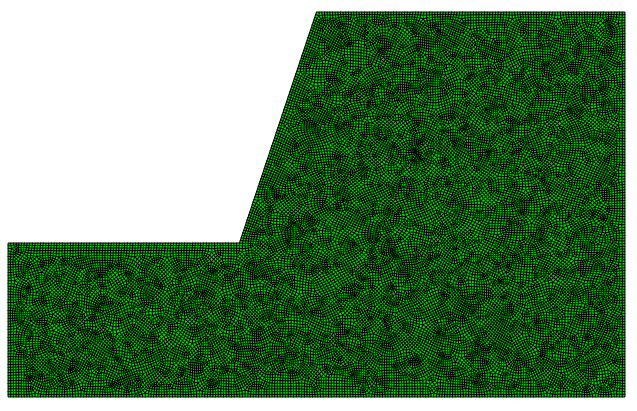
\includegraphics[width=0.6\textwidth]{figures/Chapter5/SlopeMeshNRM}
\caption{{\label{fig:SRM} Mesh for converged Drucker-Prager CDM FEM slope failure simulation
}}
\end{center}
\end{figure}

\begin{figure}[!htb]
\begin{center}
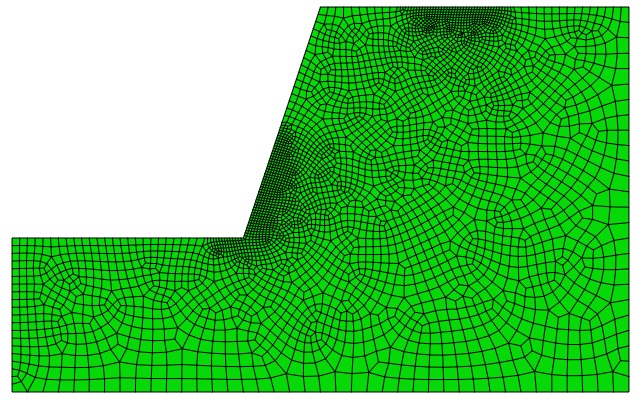
\includegraphics[width=0.6\textwidth]{figures/Chapter5/SlopeMeshSRM}
\caption{{\label{fig:NRM} Selectiverly Refined Mesh (SRM) for Drucker-Prager CDM FEM slope failure simulation.
}}
\end{center}
\end{figure}

\begin{table}[!htb]
\centering
\caption{{Comparison of Computational Time for the \glsentryshort{dns}}}
\label{tab:computation}
\begin{tabularx}{\textwidth}{@{}YYYYY@{}}
\toprule
\textbf{Simulation Type} & \textbf{Continuum Elements} & \textbf{Processor Clock Speed} & \textbf{Slope Failure Load} & \textbf{Computational Time} \\ \midrule
DEM                      & $25,898$                         & $2.20 GHz$                    & $11.2 MPa$                  & $46.5 hr$                  \\
CDM                      & $29,866$                         & $1.80 GHz$                    & $11.5 MPa$                  & $0.65 hr$                  \\
CDM - SRM                      & $3,577$                         & $1.80 GHz$                    & $11.5 MPa$                  & $0.013 hr$                  \\ \bottomrule
\end{tabularx}
\end{table}

The \acrshort{dem} simulation was run serially on a $2.2GHz$ CPU while the \acrshort{cdm} simulation was run serially on a $1.8GHz$ CPU. Despite the \acrshort{cdm} model having more continuum elements than the \acrshort{dem} model, and the \acrshort{cdm} model running on a slower CPU, a decrease in computational time of the \acrshort{dem} simulation from $46.5 hr$ to $0.65 hr$ was observed. Running the \acrshort{cdm} model with a \acrshort{srm} reduces the total computational time to $0.013 hr$, or eight minutes instead of two days. This large increase in computational efficiency with marginal decrease in model accuracy can be immensely useful for large scale geomechanical problems in \acrshort{nfr}. 
 

%----------------------------------------------------------------------
% CHAPTER 6
%----------------------------------------------------------------------
%======================================================================
\chapter{Conclusions and Future Considerations}
%======================================================================

A summary of the main conclusions from the development of the up-scaling framework as well as the implementation and testing of the framework are presented here. These conclusions represent a successful completion of the research objectives for the thesis. That being said, there are substantial limitations to this research. A series of recommendations are provided to address some of these limitations and to provide guidance on how to extend this research.

%----------------------------------------------------------------------
\section{Conclusions}
%----------------------------------------------------------------------
A multi-scale framework for up-scaling \acrshort{dem} simulations has been developed to address the computational demands of simulating microscale phenomenon in a macroscale domain in the context of NFR. Up-scaling is achieved by matching homogenized stress-strain curves from REV-scale \acrshort{dem} simulations to single element continuum models using \acrshort{pso} and LMA optimization algorithms. A Drucker-Prager plasticity model with ductile damage is implemented in the \acrshort{cdm} model to empirically capture the effect of the degradation (damage) of the NFR as deformation takes place.

\subsection*{1. Deformable DEM Homogenization}

Homogenization algorithms were developed for homogenizing \acrshort{dem} simulations with deformable bodies to assess the spatially averaged stress-strain behaviour of the REV from the microscale displacements, strains, and stresses. In this homogenization process, the resultant inter-block contact forces and block displacement from the \acrshort{dem} simulations are converted to average stresses and strains. To apply the homogenization algorithms, a method of automatically assessing a suitable REV given a sufficiently large domain was developed. These algorithms were implemented in Python\textsuperscript{TM} as the HODS software, which was used as a module for MOUSE.

\subsection*{2. Parameterization Methodology}

Two examples of the parameterization methodology are presented. Here, the key parameters required to capture the salient features of the model are isolated in order to be able to run the parameter estimation algorithms effectively. the main aspect of this parameterization methodology is the functional assumptions of the hardening/softening and damage evolution functions. In addition, the parameters are rewritten in term of physically meaningful parameters to provide more insight into the mechanics. The Drucker-Prager model with ductile damage is shown to be a reasonable \acrshort{cdm} model approach to represent NFR in a continuum context, including effects of pressure dependent yield and the triaxiality based damage initiation criterion. Compared to a full \acrshort{dem} simulation, the \acrshort{cdm} model shows a good fit pre-damage, but is unable to emulate the subtle post-yield oscillations arising from non-continuous yielding in the NFR.

\subsection*{3. Up-Scaling Framework}

MOUSE software was created and written in Python\textsuperscript{TM} to provide an implementation of the up-scaling framework presented in this thesis using in house and third-party software modules. The software itself provides a platform through which the four software elements of the up-scaling framework (\acrshort{dem} module, homogenization module, parameter estimation module, and macroscale module) can communicate with each other. The communication is facilitated by MOUSE through modules which wrap the third party software in such a way that the I/O routines to and from the modules are performed in a consistent capacity regardless of the third party software being used. A consistent set of data protocols were developed for the modules to effectively transfer data between them.

\subsection*{4. Framework Verification}

The parameter estimation module was tested and yielded an appropriate parameter set that both matched the \acrshort{dem} data and provided realistic parameters. Additionally, the Drucker-Prager model with ductile damage was found to provide a far superior fit than the damage plasticity model for quasi-brittle materials. Most importantly, the DNS of the slope stability analysis showed that with this up-scaling framework, very significant computational gains can be had with an acceptable error. Very comparable results ($<5\%$ error) to full \acrshort{dem} solutions were obtained with the \acrshort{cdm} method but required two orders of magnitude less computational time. The computational demands were again able to be reduced by another order of magnitude by using a selectively refined continuum mesh at the locations in the domain with high stress gradients.

%----------------------------------------------------------------------
\section{Recommendations}
%----------------------------------------------------------------------

The main limitation of the presented up-scaling implementation is the macroscale constitutive model module. In the current ABAQUS\textsuperscript{TM} module, the constitutive models consider only isotropic behaviour. In addition, the model does not consider the effects of pore pressure in the rock mass or fluid flow in any capacity. Though the isotropic assumptions for the elasto-plastic constitutive relationships are likely sufficiently accurate, future implementations of the macroscale constitutive model should consider anisotropic damage behaviour, as anisotropic implementations are found to be completely insufficient. In the case of the Drucker-Prager model with ductile damage, the exponential Johnson-Cook triaxiality based damage initiation criterion provides an excellent fit for monotonic loading, but does not model cyclic loading well. Here, it would be ideal for the cyclic loading capacity of the damage plasticity model for quasi-brittle materials to be incorporated as well. Ultimately, the available damage material subroutines in ABAQUS\textsuperscript{TM} are insufficient for the key physical characteristics in the system to be captured. As such, a custom anisotropic damage implementation is recommended for the macroscale constitutive model.

Retrospectively, the functional form of the hardening curve is overly complex. Though it is often necessary to model the softening of the material in the plasticity model, with \acrshort{cdm} the damage can implicitly model the softening behaviour. Here, it is observed that for the Barcelona model used for the hardening/softening curve, only the hardening portion of the curve is ever used. As such, for future implementations of the plasticity hardening functions, a simpler exponential function could be applied which would also have the benefit of decreasing the number of parameters that need to be estimated, leading to more consistent solutions and faster convergence of the optimization algorithms. 

Furthermore, it is speculated by the author that portions of the parameterization methodology could be modified to yield more consistent solutions. In the parameterization formulations presented in this thesis, too much emphasis was placed on creating physically meaningful parameters rather than numerically consistent parameters. This inconsistency is the case with certain paired parameters if one of the parameters is highly sensitive.

Additionally, effectively searching a 11+ dimensional parameter space is computationally expensive. By dividing the problem and exploiting features of the curves and constitutive models, it may be possible to increase the convergence rate and effectively get a better, faster solution. Instead of searching the entire parameter space, it is possible to split the parameters into groups (e.g. pre-damage and post damage). Here, the damage parameters don't actually affect the plasticity calculations until damage is initiated. As such, the plasticity parameters can be estimated using the pre-damage curve and the damage parameters can subsequently be estimated using the post-damage curve.

A more rigorous examination of other available optimization routines and associated optimization parameters would be another way to potentially reduce the computational cost and increase the accuracy of the parameter estimation process. \acrshort{pso} and LMA were used in this research, but Dynamically Dimensioned Search (DDS), 
Real-Coded Genetic Algorithm (RGA) and Simulated Annealing (SA) were also briefly investigated. As previously stated, rigorously assessing the most effective algorithm was not a priority of this research, but the \acrshort{pso} + LMA combination was chosen for its simplicity and effectiveness. The other algorithms, if properly applied may provide a faster and more accurate solution.
	
For this up-scaling methodology to be more accurate, 3D \acrshort{dem} simulations are required to capture accurate physical responses of these complex systems. In addition to modifying the \acrshort{dem} simulations, the associated homogenization algorithms would have to be modified to provide the 3D stress and strain tensors. 

Hydro-mechanically coupled \acrshort{dem} simulations are also an important consideration for more accurate simulations. Here, the homogenization module should be modified to assess the homogenized fluid properties such as pore pressure and flow velocity vectors and the macroscale model needs to be modified to simulate poroelastic physics.

Ultimately, rigorous validation studies should be done with real-world applications to show the viability of this approach. Incorporating some of the above reccomendations will allow this up-scaling framework to validly be applied to complex geomechanical problems in order to avoid the computational demands of \acrshort{dem} modelling.  

%----------------------------------------------------------------------
% BACK MATTER
%----------------------------------------------------------------------
\input{BackMatter}
